\documentclass{G7-32} % Стиль (по умолчанию будет 14pt)

% \usepackage{polyglossia}
% \setdefaultlanguage{russian}
% \setotherlanguage{english}

\usepackage{xurl}

\sloppy

% Overleaf compatibility switch.
% true  - skip external title PDF and use listings instead of minted
% false - use local mode with minted and Title.pdf
\newif\ifoverleafmode
\overleafmodetrue

% Настройки стиля ГОСТ 7-32
% Для начала определяем, хотим мы или нет, чтобы рисунки и таблицы нумеровались в пределах раздела, или нам нужна сквозная нумерация.
% \EqInChapter % формулы будут нумероваться в пределах раздела
% \TableInChapter % таблицы будут нумероваться в пределах раздела
% \PicInChapter % рисунки будут нумероваться в пределах раздела

% Добавляем гипертекстовое оглавление в PDF
\usepackage[
bookmarks=true, colorlinks=true, unicode=true,
urlcolor=black,linkcolor=black, anchorcolor=black,
citecolor=black, menucolor=black, filecolor=black,
]{hyperref}

\urlstyle{same}

\usepackage{pdfpages}
\usepackage[all]{hypcap}
\usepackage{needspace}

% Изменение начертания шрифта --- после чего выглядит таймсоподобно.
% apt-get install scalable-cyrfonts-tex

% \IfFileExists{cyrtimes.sty}
%     {
        % \usepackage{cyrtimespatched}
%     }
%     {
%         % А если Times нету, то будет CM...
%     }

\usepackage{graphicx}   % Пакет для включения рисунков
\graphicspath{{images/}}

% С такими оно полями оно работает по-умолчанию:
% \RequirePackage[left=20mm,right=10mm,top=20mm,bottom=20mm,headsep=0pt]{geometry}
% Если вас тошнит от поля в 10мм --- увеличивайте до 20-ти, ну и про переплёт не забывайте:

% Пакет Tikz
\usepackage{tikz}
\usetikzlibrary{arrows,positioning,shadows}

% Произвольная нумерация списков.
\usepackage{enumerate}

% ячейки в несколько строчек
\usepackage{multirow}

% itemize внутри tabular
\usepackage{paralist,array}

% Таблицы
\usepackage{array} % расширенные возможности для работы с таблицами
\usepackage{tabularx} % автоматический подбор ширины столбцов
\usepackage{dcolumn} % выравнивание чисел по разделителю

\usepackage{setspace} % полуторный интервал
\setstretch{1.43}

\newenvironment{compactlist}{%
    \renewcommand{\labelenumi}{\hspace{13mm}\arabic{enumi}.}
    \setlength{\topsep}{0pt}%
    \setlength{\partopsep}{0pt}%
    \setlength{\itemsep}{0pt}%
    \setlength{\parsep}{0pt}%
    \begin{enumerate}%
}{%
    \end{enumerate}%
}

\makeatletter
\renewcommand*\l@section{\@dottedtocline{1}{0em}{2.3em}}
\renewcommand*\l@subsection{\@dottedtocline{2}{0em}{3.2em}}
\renewcommand*\l@subsubsection{\@dottedtocline{3}{0em}{4.1em}}
\renewcommand\@dotsep{2.2}
\makeatother


\usepackage{caption}
\usepackage{ragged2e}

\DeclareCaptionJustification{centerednohyphen}{\Centering\hyphenpenalty=10000\exhyphenpenalty=10000}
\DeclareCaptionLabelSeparator{shortdash}{ \textendash\ }

\usepackage{caption}

\usepackage{float}
\setlength{\floatsep}{0pt}
\setlength{\textfloatsep}{0pt}
\setlength{\intextsep}{7pt}

\captionsetup{aboveskip=7pt,belowskip=0pt,justification=centerednohyphen,singlelinecheck=false,labelsep=shortdash}
\captionsetup[table]{justification=RaggedRight,singlelinecheck=false}
\captionsetup[figure]{justification=centerednohyphen,singlelinecheck=false,font=normalsize,labelfont=normalsize}
\captionsetup[listing]{justification=RaggedRight,singlelinecheck=false, position=top}
\captionsetup[listing]{position=top}

\usepackage{chngcntr}

\usepackage{mdframed}
\usepackage{xcolor}
\usepackage{etoolbox}

\mdfsetup{
linecolor=black,
linewidth=1pt,
roundcorner=5pt,
innerleftmargin=5pt,
innerrightmargin=5pt,
innertopmargin=5pt,
innerbottommargin=5pt,
skipabove=0pt, % Reduces space above the frame
skipbelow=0pt, % Reduces space below the frame
leftmargin=0pt, % Reduces left outer margin
rightmargin=0pt % Reduces right outer margin
}

\ifoverleafmode
  \usepackage{listings}
  \usepackage{newfloat}
  \DeclareFloatingEnvironment[
    fileext=lol,
    listname={Листинги},
    name=Листинг
  ]{listing}
  \lstset{
      basicstyle=\ttfamily\small,
      numbers=left,
      numberstyle=\scriptsize\color{gray},
      numbersep=8pt,
      breaklines=true,
      breakatwhitespace=false,
      columns=fullflexible,
      keepspaces=true,
      showstringspaces=false,
      xleftmargin=2.4em,
      framexleftmargin=2.0em,
      tabsize=2,
      backgroundcolor=\color{black!3},
      keywordstyle=\color{blue!70!black}\bfseries,
      commentstyle=\color{green!45!black}\itshape,
      stringstyle=\color{red!65!black}
  }
  \lstnewenvironment{minted}[2][]{
    \lstset{
      language=#2,
      #1
    }
  }{}
  \newcommand{\inputminted}[3][]{\lstinputlisting[language=#2,#1]{#3}}
\else
  \usepackage[chapter]{minted}
  \usemintedstyle{friendly}

  % Configure captions for minted's listing environment
  \captionsetup[listing]{
      position=top,
      justification=RaggedRight,
      singlelinecheck=false
  }

  % Alternative: Force all float captions to top
  \floatstyle{plaintop}
  \restylefloat{listing}

  \setminted{
      linenos=true,           % включить номера строк
      numberblanklines=false, % не нумеровать пустые строки
      numbersep=5pt,          % расстояние между номерами строк и кодом
      xleftmargin=1em,        % отступ слева, чтобы номера не вылезали за границы
      fontsize=\small,
      breakanywhere=true,
      breakautoindent=true,
      breaklines=true,
      bgcolor=black!3,
  }

  \renewcommand{\listingscaption}{Листинг}
  \renewcommand{\listoflistingscaption}{Листинги}
\fi


\makeatletter
\let\oldtableofcontents\tableofcontents
\renewcommand{\tableofcontents}{%
  \begingroup
  \hyphenpenalty=10000
  \exhyphenpenalty=10000
  \oldtableofcontents
  \endgroup
}
\makeatother

\makeatletter
\def\@hangfrom#1{\setbox\@tempboxa\hbox{{#1}}%
      \hangindent 0pt%\wd\@tempboxa
      \noindent\box\@tempboxa}
\makeatother

\ifoverleafmode\else
\AtEndEnvironment{listing}{\vspace{-4pt}}
\fi
\AtEndEnvironment{table}{\vspace{0pt}}
\AtEndEnvironment{center}{\vspace{0pt}}
\AtEndEnvironment{figure}{\vspace{0pt}}


\usepackage{fontspec}

% Указываем шрифты для основного текста и для кириллицы:
\setmainfont{Times New Roman} % если установлен в системе
\newfontfamily\cyrillicfont{Times New Roman} % для кириллического текста

% Убирает точку после номера главы
\makeatletter
\renewcommand{\thesection}{\thechapter.\arabic{section}}
\renewcommand{\thesubsection}{\thesection.\arabic{subsection}}
\renewcommand{\@seccntformat}[1]{%
  {\fontsize{14pt}{21pt}\selectfont\bfseries \csname the#1\endcsname}\hspace{1em}%
}
\makeatother

% Keep normal spacing after section titles.
\setlength\GostAfterTitleSkip{3.2ex}

% Remove bottom spacing for second-level headings (\section).
\makeatletter
\renewcommand\section{%
 \@afterindenttrue
 \@startsection{section}{1}%
 {\GostTitleIndent}{\GostBeforTitleSkip}{0.6ex}%
 {\GostTitleStyle}%
}
\makeatother


\begin{document}

\frontmatter % выключает нумерацию ВСЕГО; здесь начинаются ненумерованные главы: реферат, введение, глоссарий, сокращения и прочее.

% Команды \breakingbeforechapters и \nonbreakingbeforechapters
% управляют разрывом страницы перед главами.
% По-умолчанию страница разрывается.

% \nobreakingbeforechapters
% \breakingbeforechapters
\ifoverleafmode
% Title PDF is disabled for Overleaf mode.
\else

\includepdf[pages={1-5}]{./extra/Title.pdf}
\fi


\begin{abstract}
\thispagestyle{empty}

Выпускная квалификационная работа выполнена на тему: <<Веб-приложение для планирования питания с учетом предпочтений пользователей>>.

Назначение разработанного программного продукта состоит в автоматизации планирования рациона питания, формировании устойчивых здоровых пищевых привычек и повышении эффективности составления меню в повседневной практике пользователей.

Основные функции разработанного веб-приложения:
\begin{compactlist}
  \item автоматический расчет пищевой ценности для каждого рецепта;
  \item составление персональных планов питания на день, неделю или месяц (ручной и автоматический подбор);
  \item формирование списка покупок на основе выбранных рецептов;
  \item интеллектуальный ассистент для консультаций по питанию;
  \item аналитика пищевых привычек и прогресса достижения пользовательских целей.
\end{compactlist}

В работе используются следующие технологии: PostgreSQL (база данных), Python и Django (серверная часть), React и Effector (клиентская часть).

Работа включает введение, три главы, заключение, список использованных источников и приложения.

Во введении обоснована актуальность темы, сформулированы цель и задачи, определены объект и предмет исследования, а также практическая значимость результатов. В первой главе рассмотрена предметная область, проведен анализ целевой аудитории, ролевой модели и конкурентных решений, сформулированы требования к системе и обоснован выбор технологического стека. Во второй главе представлена реализация программного решения: проектирование структуры данных, разработка клиентской части, серверной части и прикладных модулей (планирование, расчет КБЖУ, модерация, уведомления). В третьей главе описаны тестирование, контейнеризация и порядок развертывания системы.

Практический результат ВКР --- работоспособное веб-приложение для планирования питания с поддержкой персонализации, автоматизации рутинных операций и ролевого управления контентом.

Практическая значимость разработанного решения состоит в снижении трудозатрат на составление рациона, повышении прозрачности контроля пищевой ценности и упрощении формирования списка покупок. Разработанная система может использоваться как самостоятельный цифровой инструмент для частных пользователей и как основа для дальнейшего развития сервисов в сфере здорового питания.
\end{abstract}

\tableofcontents

\Introduction

Вопросы, связанные с питанием и профилактикой неинфекционных заболеваний, являются устойчивым направлением исследований в сфере общественного здоровья. По данным Всемирной организации здравоохранения, факторы образа жизни, включая питание, рассматриваются как значимая составляющая профилактики и снижения риска хронических заболеваний \cite{who2025stats}. В этой связи востребованы цифровые инструменты, позволяющие системно организовывать рацион и снижать долю рутинных операций при его планировании.

Целью выпускной квалификационной работы является разработка веб-приложения для планирования питания с учетом предпочтений пользователей.

Для достижения поставленной цели необходимо решить следующие задачи:
\begin{compactlist}
  \item исследовать предметную область;
  \item определить функции продукта и технологии разработки;
  \item проанализировать целевую аудиторию;
  \item проанализировать аналоги и конкурентов;
  \item спроектировать структуру базы данных;
  \item спроектировать интерфейс;
  \item разработать клиентскую часть;
  \item разработать серверную часть;
  \item разработать модули проверки макета и расчета стоимости;
  \item разместить веб-сервис на сервере.
\end{compactlist}

Объект исследования --- процесс планирования питания, включающий подбор рецептов, учет пользовательских ограничений, расчет пищевой ценности, формирование планов питания и связанных с ними списков покупок.

Предмет исследования --- методы и программные средства автоматизации планирования питания в формате веб-приложения.

Практическая значимость работы состоит в создании прикладного решения, позволяющего пользователю сократить время на планирование рациона, повысить прозрачность контроля КБЖУ и упростить формирование меню и списка покупок.



\mainmatter % это включает нумерацию глав и секций в документе ниже
\setcounter{secnumdepth}{1} % максимум: глава.раздел (например, 1.2)
\setcounter{tocdepth}{1} % в оглавлении до уровня разделов

\chapter{{\fontsize{14pt}{21pt}\selectfont\MakeUppercase{Предметная область и технологии}}}
\label{cha:analysis}

\section{Исследование предметной области}

На начальном этапе разработки рассмотрен практический сценарий пользователя, который стремится планировать рацион системно: подбирать рецепты, учитывать ограничения по питанию, формировать меню на период и получать список покупок. Анализ существующих пользовательских сценариев показывает, что эти действия часто распределены между несколькими сервисами: кулинарными порталами, приложениями учета калорий и отдельными инструментами ведения заметок.

При таком подходе возникают повторяющиеся операционные трудности: дублирование данных, ручной перенос информации между сервисами, отсутствие единой модели пользовательских предпочтений и ограничений, а также разрыв между этапом выбора блюда и этапом практического исполнения плана (покупка продуктов). В результате возрастает время на планирование и снижается управляемость процесса в долгосрочном периоде.

Предварительный обзор существующих решений показывает, что на рынке присутствуют как кулинарные платформы, так и специализированные сервисы учета питания, однако пользовательский сценарий часто остается разорванным между несколькими инструментами \cite{nutristeppe_diaries_2026,institutfitnesa_apps_2026,sportmaster_apps_2026}. Детальный сравнительный анализ конкурентов и аналогов приведен в разделе~1.4.

\section{Определение целевой аудитории}

Целевая аудитория разрабатываемого веб-приложения включает группы пользователей, объединенные общей потребностью в системном управлении питанием, но различающиеся по сценариям использования.

Основная пользовательская аудитория

К основной аудитории относятся пользователи, планирующие рацион в соответствии с персональными целями:
\begin{compactlist}
  \item снижение массы тела, поддержание формы или набор массы;
  \item учет персональных ограничений в питании;
  \item ускорение ежедневного планирования меню;
  \item получение рекомендаций по выбору блюд и структуры рациона.
\end{compactlist}

Ключевые требования этой группы:
\begin{compactlist}
  \item персонализация рекомендаций и фильтрации;
  \item визуально понятное планирование по дням и приемам пищи;
  \item контроль КБЖУ и состава блюд \cite{sektascience_bzhu_2026};
  \item формирование практического списка покупок на основе выбранного меню.
\end{compactlist}

Авторы пользовательского контента

В данную группу входят пользователи, которые создают рецепты, публикуют планы питания и оставляют отзывы.

Для этой категории критичны:
\begin{compactlist}
  \item удобные формы публикации и редактирования материалов;
  \item прозрачность статусов модерации контента;
  \item получение обратной связи от других пользователей.
\end{compactlist}

Ролевые группы в системе

Ролевые группы описывают не целевую аудиторию, а модель разграничения прав доступа в программной системе.

Пользователь

Базовая роль, обеспечивающая работу с рецептами, планами питания, отзывами, избранным и списками покупок в рамках собственных данных.

Модератор

Роль контроля качества контента: проверка рецептов, отзывов и жалоб, принятие решений по модерации, корректировка публикаций в пределах регламента платформы.

Администратор

Роль расширенного системного управления: управление учетными записями и ролями, администрирование справочников, контроль устойчивости и безопасности функционирования платформы.

\section{Проектирование бизнес-процессов}

Бизнес-процесс представляет собой совокупность связанных активностей, преобразующих входные данные в результат, имеющий ценность для пользователя \cite{kirillina_bpm_2022}. Для формализации процессов в рамках проекта используется подход структурного анализа и проектирования SADT (Structured Analysis and Design Technique), в составе которого применяется семейство нотаций IDEF \cite{mindalev_idef_2016,sadt_intro_ross,idef0_fips_183}.

Краткая характеристика основных нотаций IDEF приведена в таблице~\ref{tab:idef-notations}.

\begin{table}[H]
\caption{Краткая характеристика нотаций IDEF}
\label{tab:idef-notations}
\small
\begin{tabularx}{\textwidth}{|p{0.16\textwidth}|p{0.30\textwidth}|X|}
\hline
\multicolumn{1}{|c|}{Нотация} & \multicolumn{1}{c|}{Назначение нотации} & \multicolumn{1}{c|}{Основные отражаемые объекты} \\ \hline
IDEF0 & Создание функциональной модели & Функции, входы/выходы, управляющие воздействия и механизмы выполнения процессов. \\ \hline
IDEF1 & Построение информационной модели & Информационные потоки и структура данных предметной области. \\ \hline
IDEF1X & Построение реляционных структур & Сущности, атрибуты и связи между сущностями в терминах реляционной модели. \\ \hline
IDEF3 & Документирование сценариев выполнения процессов & Последовательность операций и варианты прохождения процесса. \\ \hline
IDEF5 & Онтологическое описание сложных систем & Классы объектов, отношения, ограничения и изменения состояния. \\ \hline
\end{tabularx}
\normalsize
\end{table}

Для проектирования ключевого процесса <<Составление плана питания пользователем>> в проекте использована нотация IDEF0, а для описания межролевого взаимодействия --- BPMN 2.0 \cite{mindalev_idef_2016,zueva_bpmn_2021,bpmn_spec_2014}.

Нотация BPMN 2.0 поддерживает несколько типов представлений: оркестровка (один пул с внутренним потоком управления), диаграмма взаимодействия (несколько пулов и обмен сообщениями), хореография и схема диалога \cite{zueva_bpmn_2021,bpmn_spec_2014}. В рамках FoodPlanner практическую ценность для описания пользовательских и системных сценариев имеют оркестровка и диаграмма взаимодействия.

Диаграмма вариантов использования на \hyperref[fig:uml-users]{рисунке~\ref*{fig:uml-users}} показывает распределение сценариев между ролями системы.

\begin{figure}[H]
  \centering
  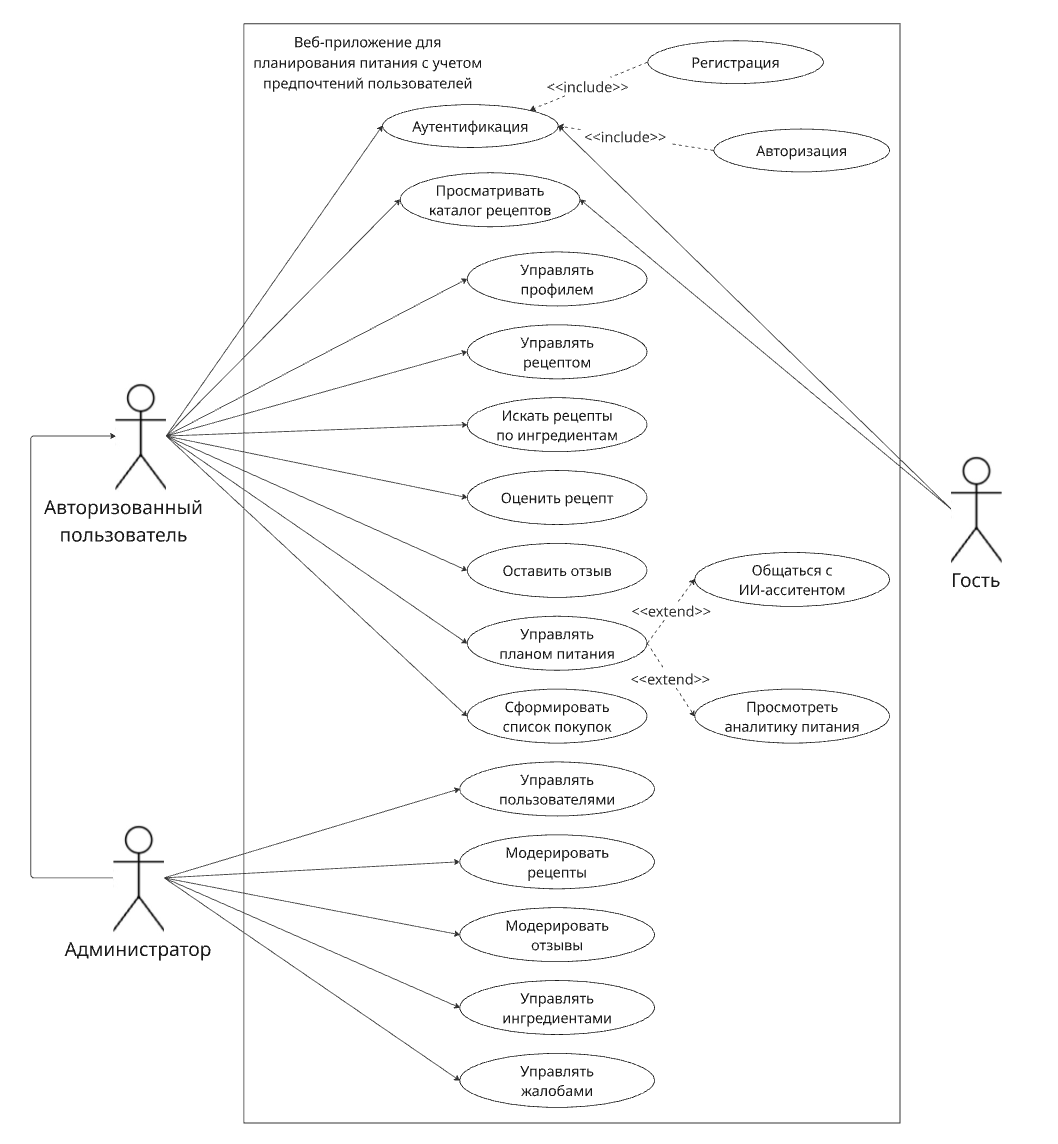
\includegraphics[width=0.95\textwidth]{UML.png}
  \caption{UML-диаграмма пользователей}
  \label{fig:uml-users}
\end{figure}

Неавторизованный пользователь (гость) имеет доступ к просмотру каталога рецептов и регистрации в системе. После прохождения регистрации пользователь получает возможность авторизации и перехода к персональным сценариям.

Авторизованный пользователь, помимо просмотра каталога, может редактировать профиль, указывать предпочтения, создавать и редактировать собственные рецепты, собирать планы питания, формировать список покупок, оставлять оценки и отзывы, а также использовать ИИ-ассистента и просматривать персональную аналитику.

Администратор обеспечивает управленческие и контрольные функции: управление пользователями и ролями, администрирование справочников, контроль жалоб и контроль корректности модерационных процессов.

Процесс взаимодействия пользователя с планом питания представлен BPMN-диаграммой (\hyperref[fig:bpmn-plan-interaction]{рисунок~\ref*{fig:bpmn-plan-interaction}}).

\begin{figure}[H]
  \centering
  \IfFileExists{images/bpmn-plan-interaction.png}{
    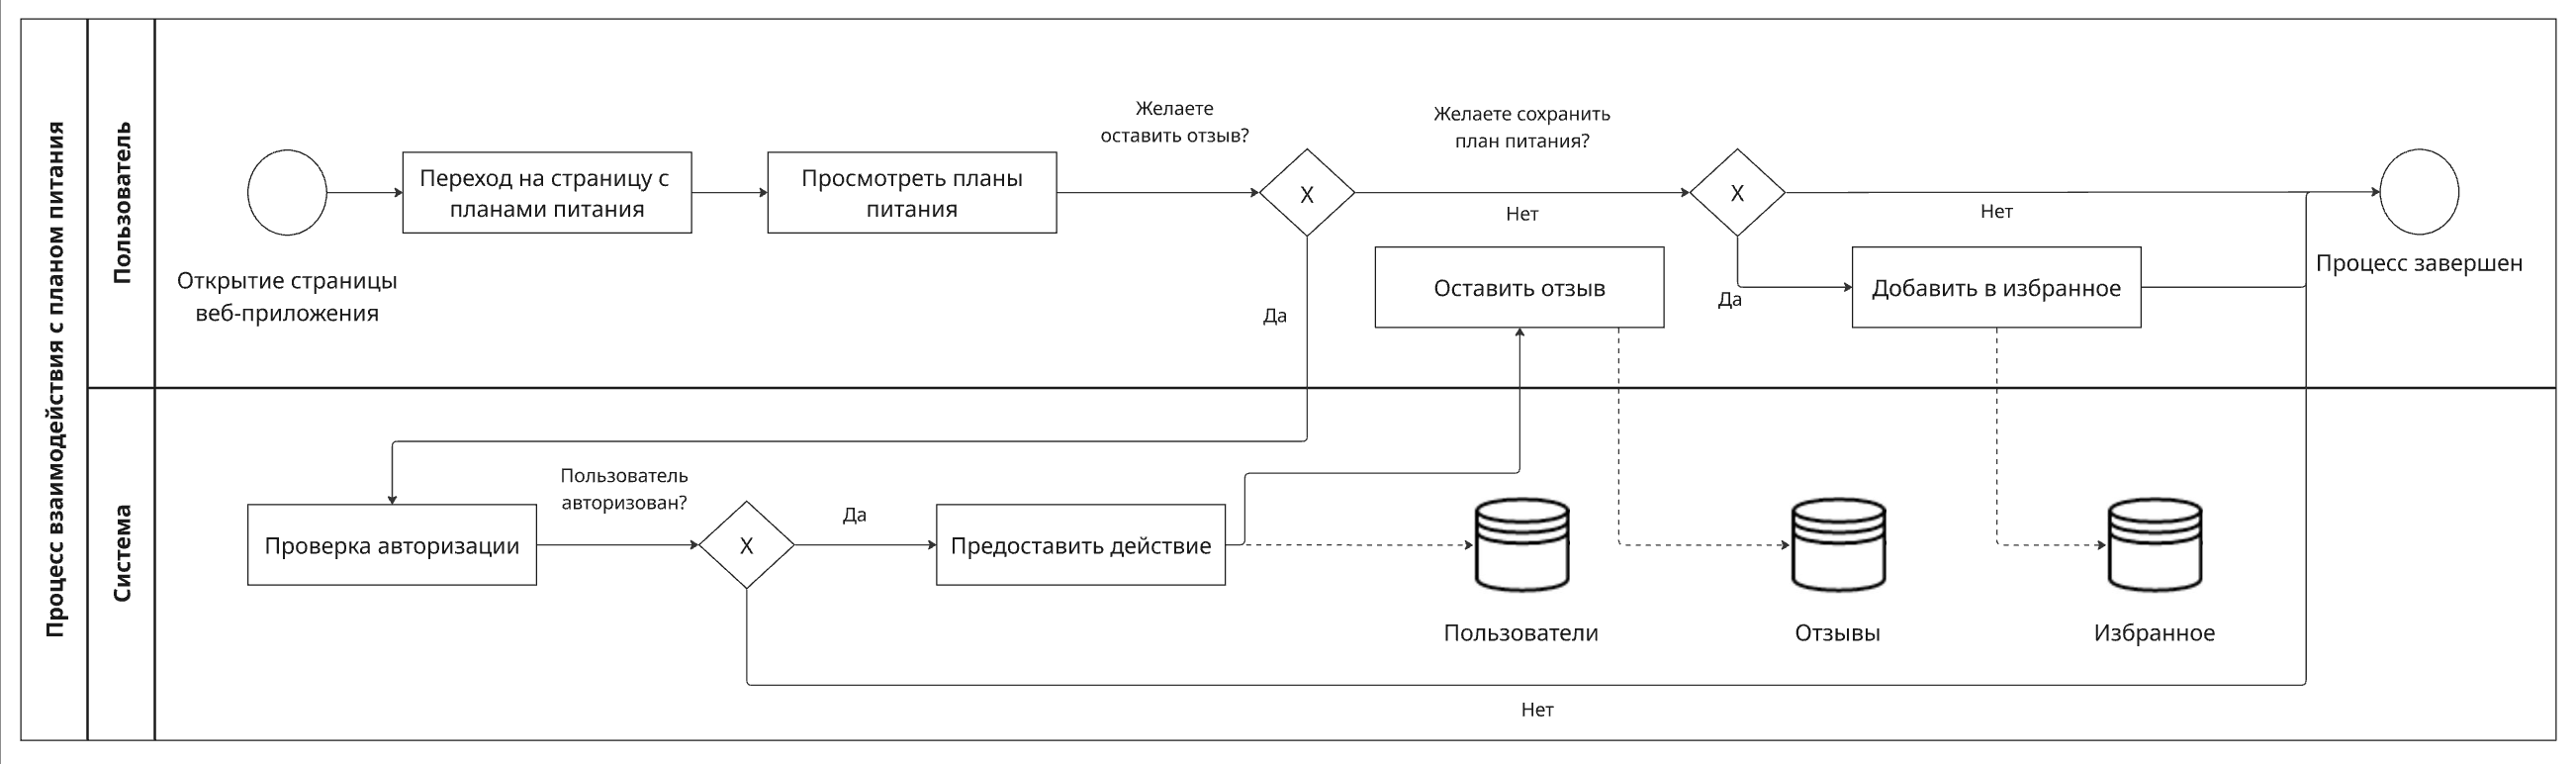
\includegraphics[angle=90,width=\textwidth,height=0.90\textheight,keepaspectratio]{bpmn-plan-interaction.png}
  }{
    \fbox{\parbox{0.9\textwidth}{\centering Место для рисунка BPMN\\
    Файл: \texttt{Report/images/bpmn-plan-interaction.png}}}
  }
  \caption{BPMN-диаграмма процесса взаимодействия пользователя с планом питания}
  \label{fig:bpmn-plan-interaction}
\end{figure}

Алгоритм составления плана питания пользователем приведен на \hyperref[fig:plan-creation-process]{рисунке~\ref*{fig:plan-creation-process}}.

\begin{figure}[H]
  \centering
  \IfFileExists{images/plan-creation-process.png}{
    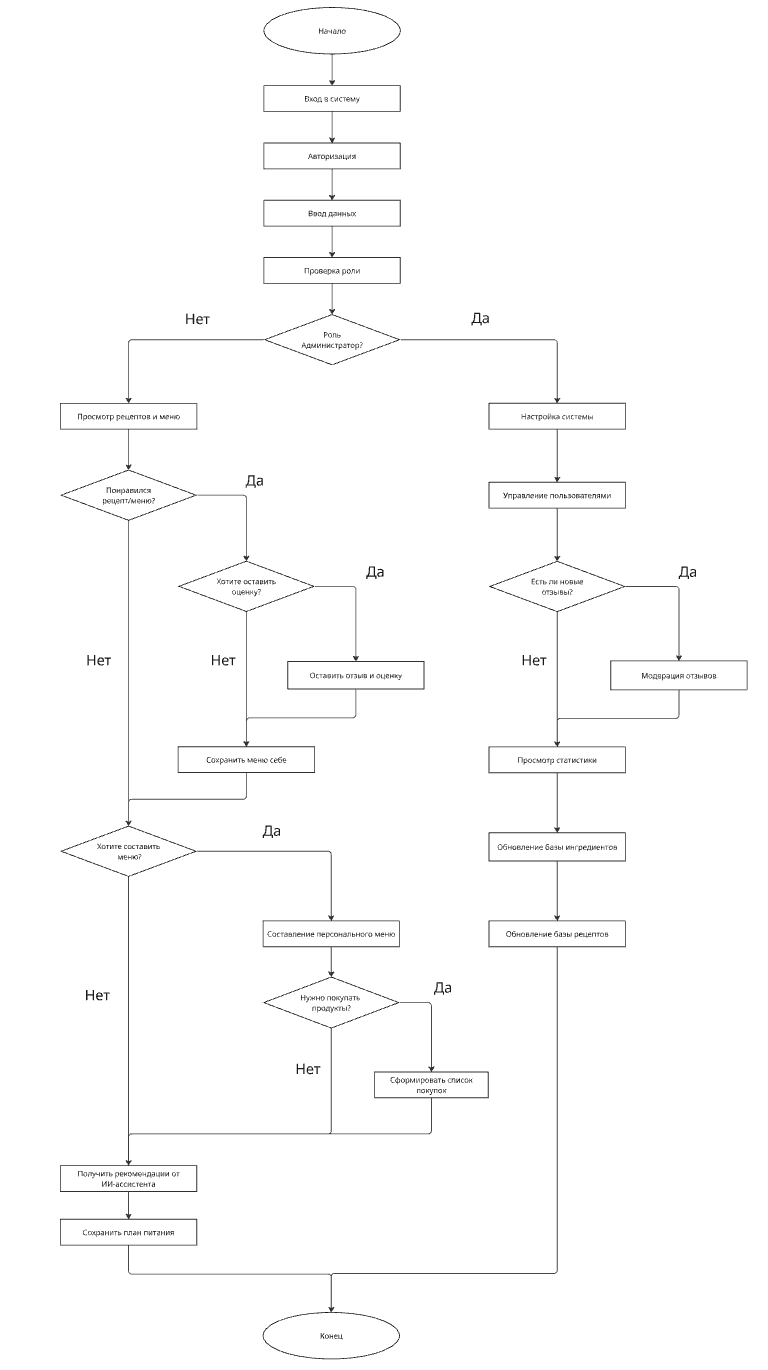
\includegraphics[width=\textwidth,height=0.88\textheight,keepaspectratio]{plan-creation-process.png}
  }{
    \fbox{\parbox{0.9\textwidth}{\centering Место для рисунка процесса\\
    Файл: \texttt{Report/images/plan-creation-process.png}}}
  }
  \caption{Процесс создания плана питания}
  \label{fig:plan-creation-process}
\end{figure}

\textbf{Взаимодействие пользователя с системой в рамках IDEF0}

Пользователь задает исходные условия: доступные продукты, цели питания, ограничения и предпочтения. Эти данные поступают на вход функциональной модели. Далее система последовательно выполняет анализ входных данных, подбор рецептов, формирование меню и генерацию списка покупок с расчетом пищевой ценности.

Контекстная диаграмма IDEF0 (уровень A-0)

На контекстном уровне система представлена единой функцией <<Планирование питания с учетом предпочтений пользователя>>. Входами являются данные о продуктах и целях питания; управлениями --- ограничения, предпочтения и нормативные параметры; механизмами --- веб-интерфейс, сервер приложений и база данных; выходами --- сформированное меню, список покупок и расчет пищевой ценности.

Декомпозиция IDEF0 (уровень A0)

Декомпозиция верхнего уровня включает четыре функциональных блока:
\begin{compactlist}
  \item анализ имеющихся продуктов;
  \item поиск подходящих рецептов;
  \item выбор оптимального меню на период;
  \item формирование списка недостающих покупок.
\end{compactlist}

Диаграммы IDEF0 и IDEF1 приведены на \hyperref[fig:idef0]{рисунке~\ref*{fig:idef0}} и \hyperref[fig:idef1]{рисунке~\ref*{fig:idef1}}.

\begin{figure}[H]
  \centering
  \IfFileExists{images/idef0.png}{
    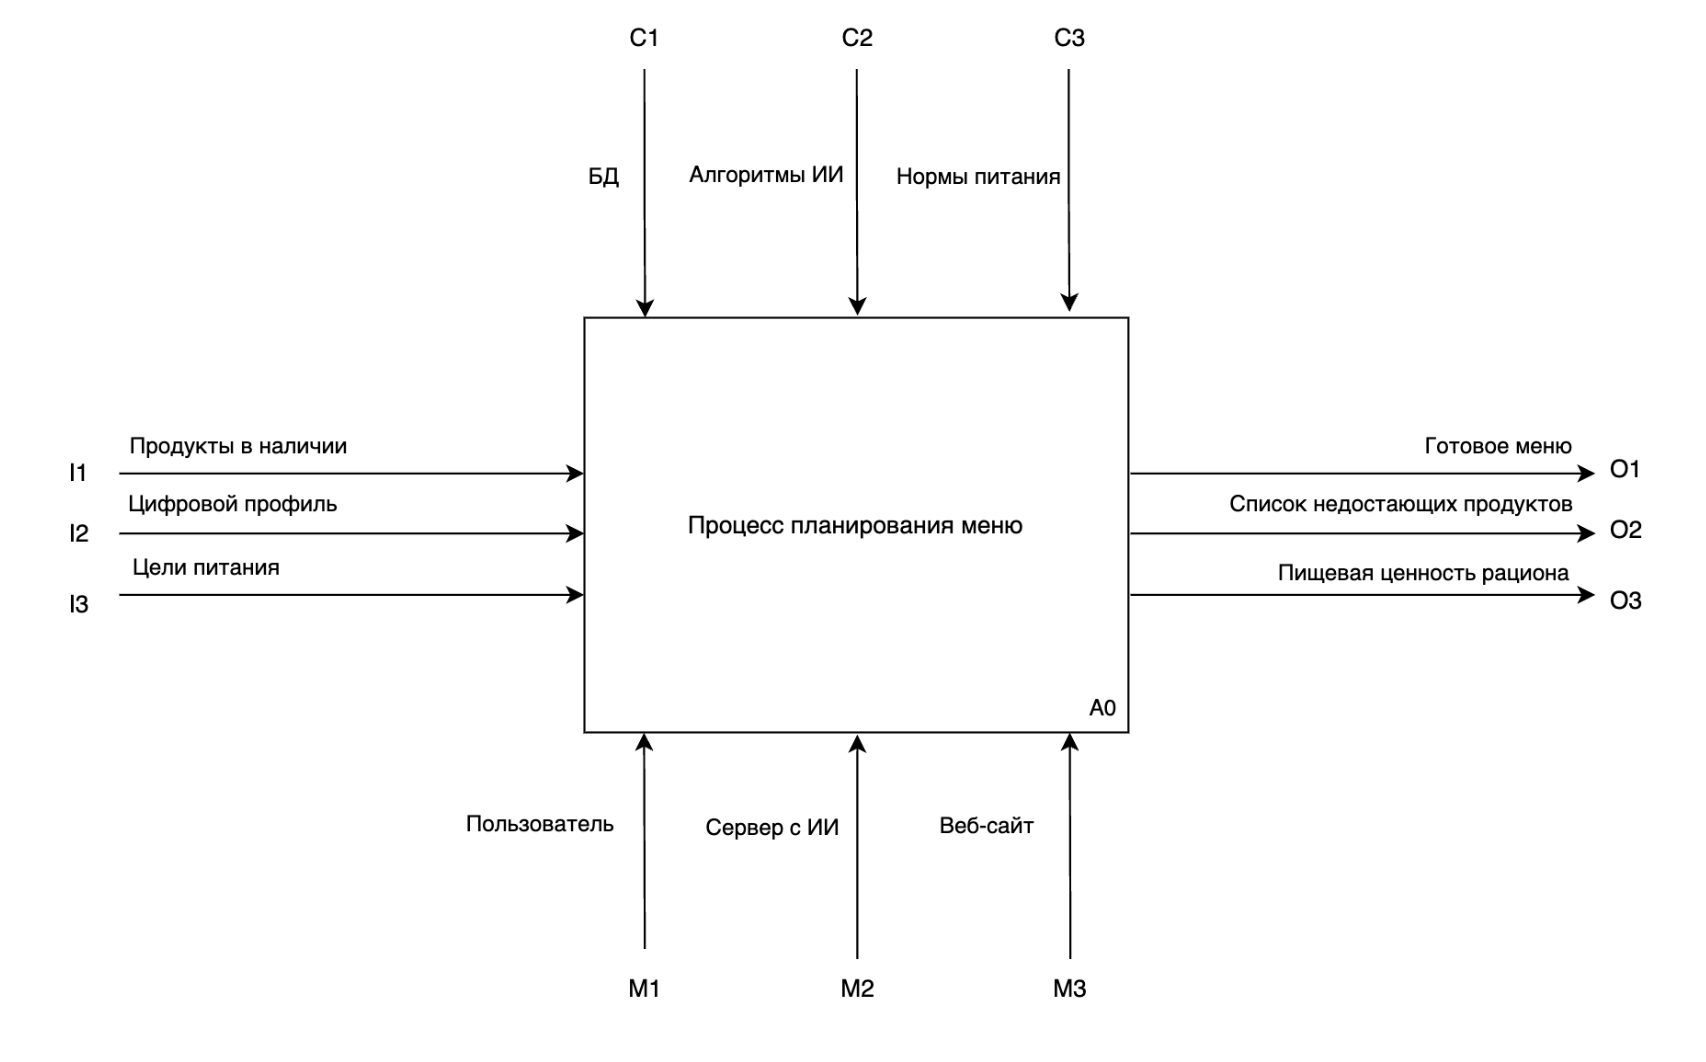
\includegraphics[angle=90,width=\textwidth,height=0.90\textheight,keepaspectratio]{idef0.png}
  }{
    \fbox{\parbox{0.9\textwidth}{\centering Место для диаграммы IDEF0\\
    Файл: \texttt{Report/images/idef0.png}}}
  }
  \caption{IDEF0-диаграмма бизнес-процесса}
  \label{fig:idef0}
\end{figure}

\begin{figure}[H]
  \centering
  \IfFileExists{images/idef1.png}{
    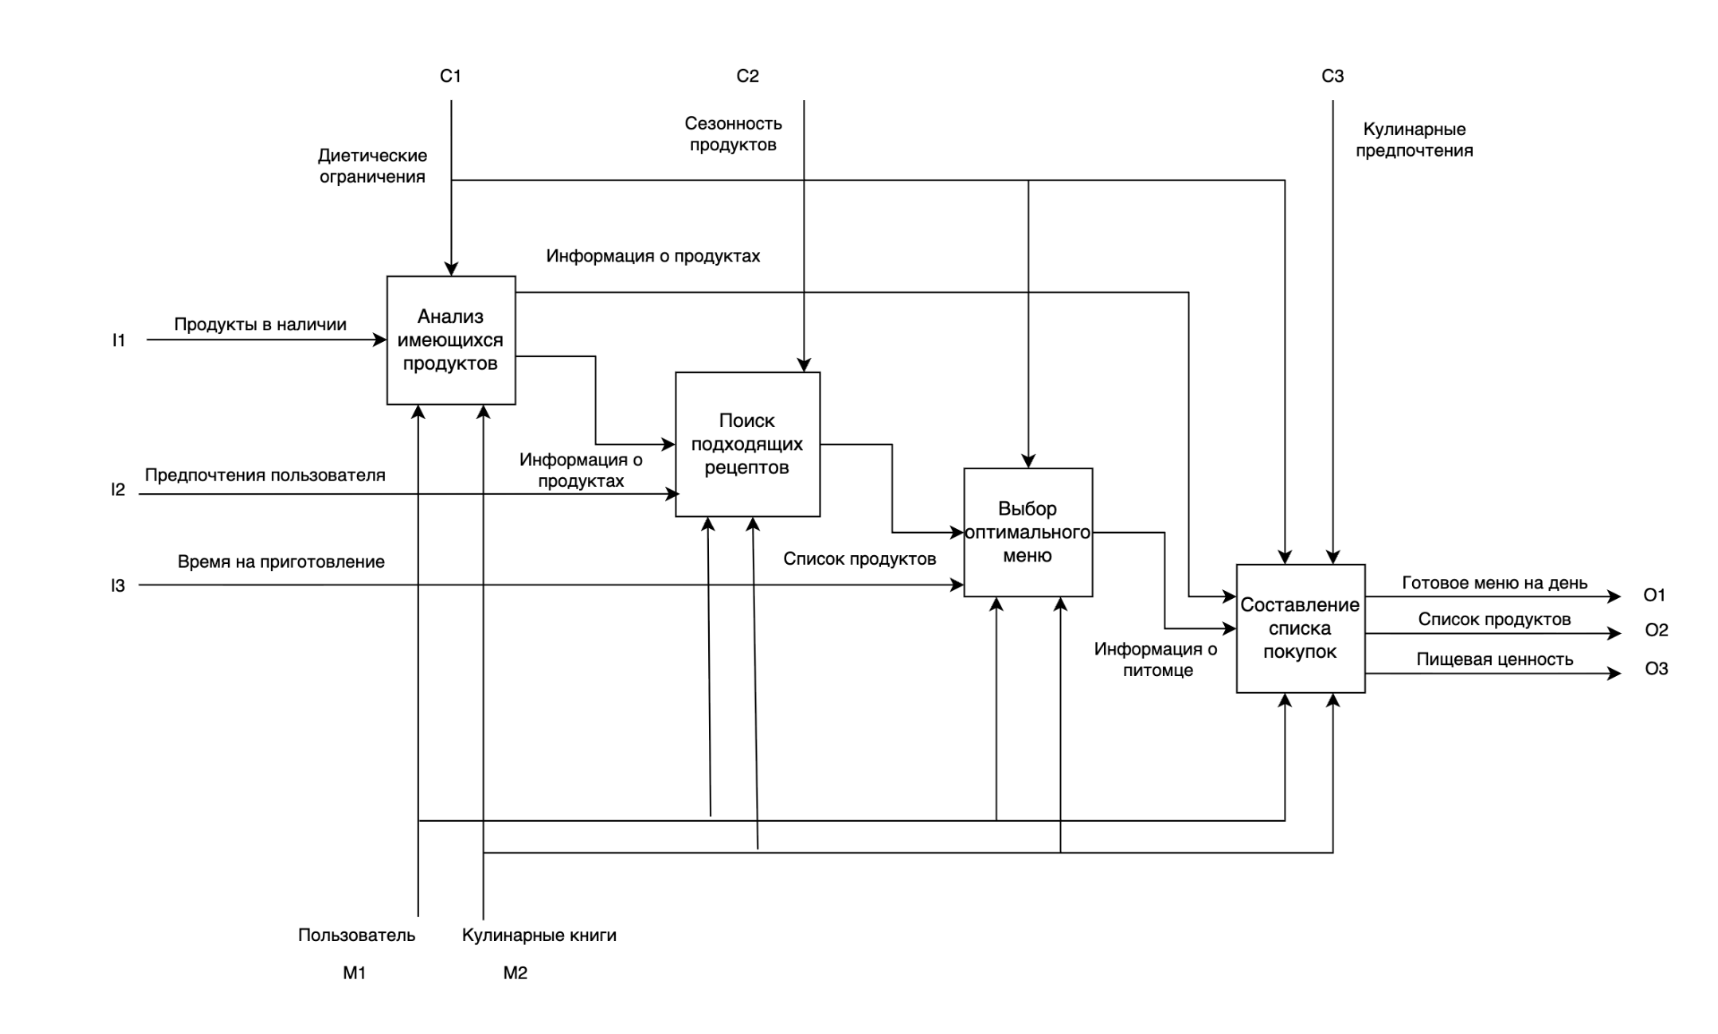
\includegraphics[angle=90,width=\textwidth,height=0.90\textheight,keepaspectratio]{idef1.png}
  }{
    \fbox{\parbox{0.9\textwidth}{\centering Место для диаграммы IDEF1\\
    Файл: \texttt{Report/images/idef1.png}}}
  }
  \caption{IDEF1-диаграмма структуры данных}
  \label{fig:idef1}
\end{figure}

\section{Анализ аналогов и конкурентов}

Анализ аналогов и конкурентов выполнен для оценки уровня покрытия пользовательских потребностей, выявленных в предыдущих разделах: целостное планирование рациона, персонализация, учет ограничений, формирование списка покупок и поддержка модерации пользовательского контента. Дополнительно учтены обзорные публикации по приложениям и дневникам питания \cite{nutristeppe_diaries_2026,institutfitnesa_apps_2026,sportmaster_apps_2026}.

В качестве конкурентов и функциональных аналогов выбраны платформы, которые наиболее близки к сценарию FoodPlanner по пользовательским задачам: MenuBook, <<Еда>>, Ovkuse, <<Поварёнок>> и MyFitnessPal \cite{menubook2026,eda2026,ovkuse2026,povarenok2026,myfitnesspal2026}. Для оценки использовались следующие критерии: наличие конструктора плана питания, учет пищевых предпочтений, ИИ-помощник, доступность базового функционала без подписки, качество пользовательского интерфейса и наличие сообщества.

\begin{table}[H]
\caption{Сравнение конкурентов и аналогов}
\label{tab:analog-competitors}
\small
\begin{tabular}{|p{0.18\textwidth}|p{0.28\textwidth}|p{0.46\textwidth}|}
\hline
\multicolumn{1}{|c|}{Сервис} & \multicolumn{1}{c|}{Сильные стороны} & \multicolumn{1}{c|}{Ограничения для целевого сценария} \\ \hline
MenuBook & Праздничные сценарии меню, расчет ИМТ, базовые рекомендации, очень хорошее создание плана питания & Нет ИИ-ассистента; значимая часть сценариев платная; нет полноценного подбора по предпочтениям. \\ \hline
Еда (Rambler) & Сильный визуал, модерация рецептов, развитый контентный раздел & Нет конструктора плана питания, слабая персонализация по ограничениям, нет ИИ-ассистента. \\ \hline
Ovkuse & Большая рецептная база, активное сообщество, есть ИИ-ассистент & Много полезных функций доступно только по подписке; нет полноценного конструктора длительного плана питания. \\ \hline
Поварёнок & Крупная база рецептов, БЖУ, дневники, Q\&A, посты и видео & Устаревший интерфейс; нет ИИ-помощника и нет конструктора плана питания в целевом формате. \\ \hline
MyFitnessPal & Сильный онбординг по целям, трекинг прогресса, дэшборды & Фокус на учете и фитнесе; нет ИИ и нет гибкого конструктора меню по дням и приемам пищи. \\ \hline
\end{tabular}
\normalsize
\end{table}

MenuBook \cite{menubook2026} демонстрирует сильный сценарий подготовки меню под конкретный формат питания: пользователь может собирать меню, в том числе для специальных и праздничных случаев, а также получать базовые рекомендации и расчет индекса массы тела. Интерфейс сервиса ориентирован на быстрый переход к готовым сценариям, что упрощает вход для широкой аудитории. Вместе с тем платформа не предлагает встроенного ИИ-ассистента и не закрывает полноценный сценарий персонализации по ограничениям и предпочтениям пользователя. Интерфейс платформы MenuBook представлен на рисунке~\ref{fig:competitor-menubook}.

\begin{figure}[H]
  \centering
  \IfFileExists{images/competitor-menubook.png}{
    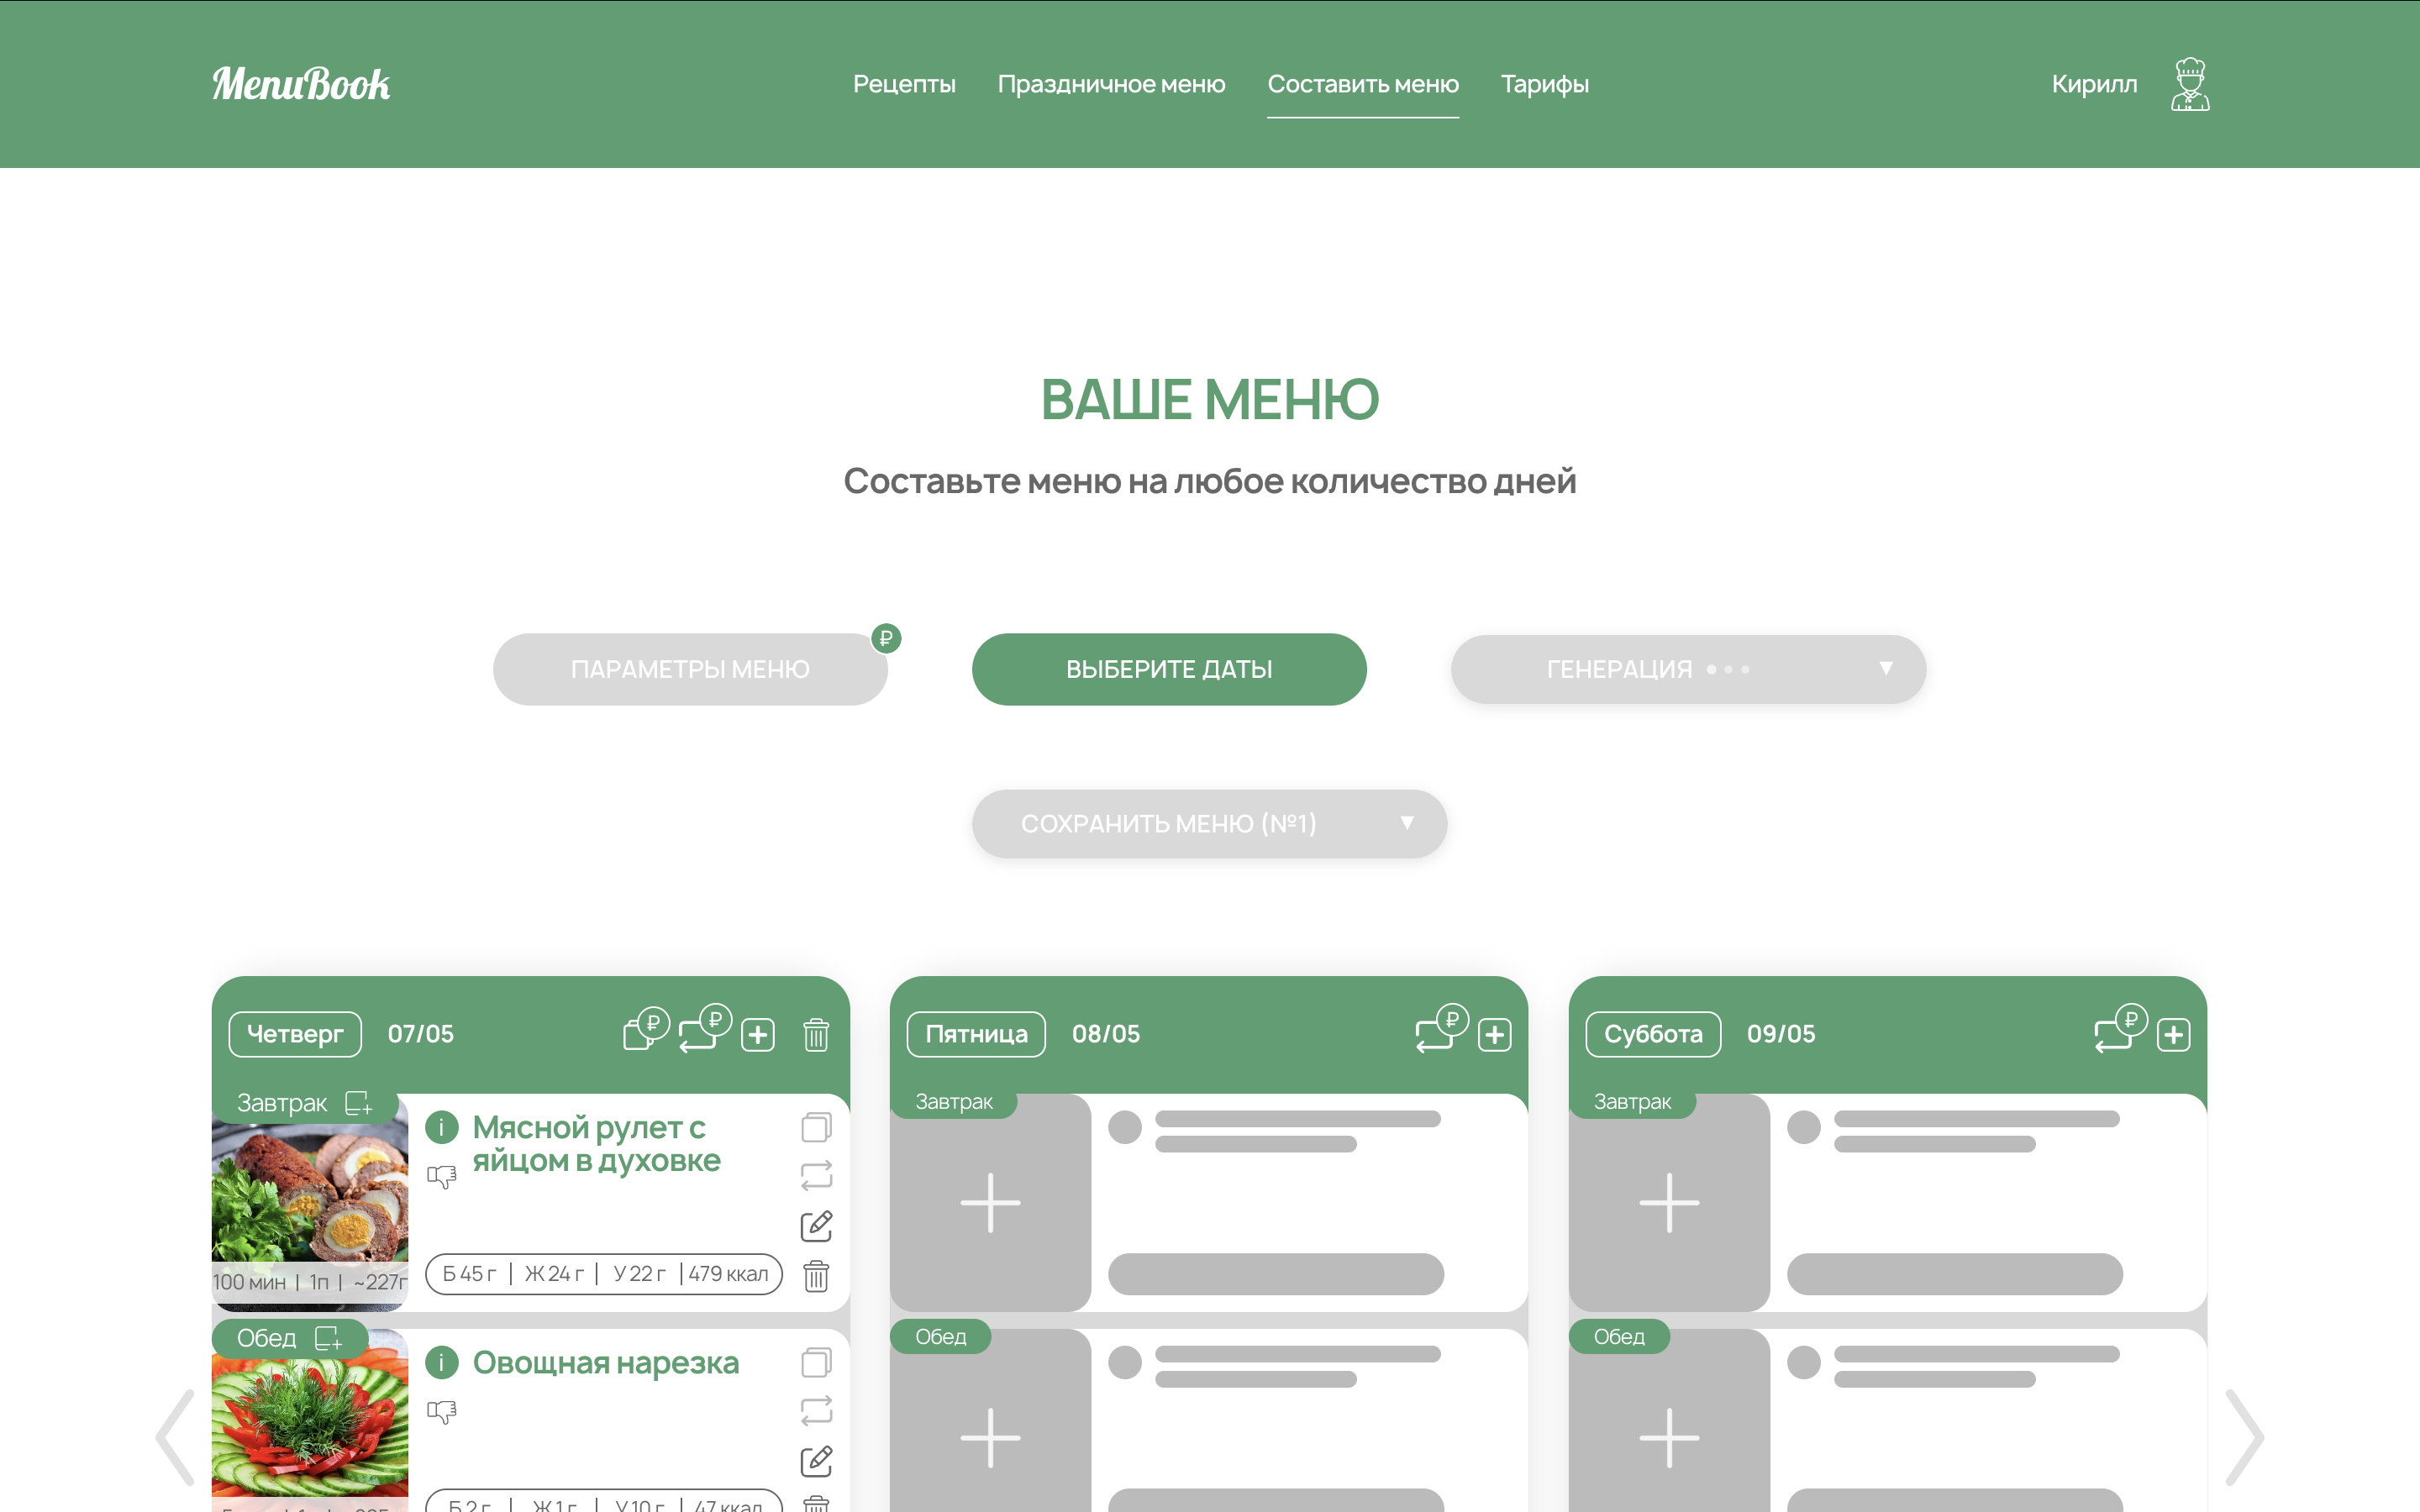
\includegraphics[width=\textwidth,height=0.82\textheight,keepaspectratio]{images/competitor-menubook.png}
  }{
    \fbox{\parbox{0.92\textwidth}{\centering Файл скриншота не найден: \texttt{images/competitor-menubook.png}}}
  }
  \caption{Интерфейс платформы MenuBook}
  \label{fig:competitor-menubook}
\end{figure}

Платформа <<Еда>> \cite{eda2026} показывает высокий уровень контентного качества и редакционного сопровождения: пользователь получает широкий выбор рецептов, статей и тематических подборок с удобной навигацией. Важным плюсом является зрелая контентная экосистема и стабильные пользовательские сценарии входа, что повышает удобство ежедневного использования. Однако основной фокус сервиса остается информационно-рецептурным, а не планировочным: отсутствует конструктор рациона и выраженная персонализация по пищевым ограничениям. Интерфейс платформы <<Еда>> представлен на рисунке~\ref{fig:competitor-eda-rambler}.

\begin{figure}[H]
  \centering
  \IfFileExists{images/competitor-eda-rambler.png}{
    
\includegraphics[width=\textwidth,height=0.82\textheight,keepaspectratio]{images/competitor-eda-rambler.png}
  }{
    \fbox{\parbox{0.92\textwidth}{\centering Файл скриншота не найден: \texttt{images/competitor-eda-rambler.png}}}
  }
  \caption{Интерфейс платформы Еда (Rambler)}
  \label{fig:competitor-eda-rambler}
\end{figure}

Ovkuse \cite{ovkuse2026} интересен сочетанием активного сообщества, большой базы рецептов и наличием ИИ-ассистента для быстрого подбора блюд. Сервис также предлагает расширенные сценарии просмотра и дополнительные блоки данных по рациону, что может быть полезно для вовлеченных пользователей. При этом значимая часть практической функциональности для регулярного использования переведена в подписочную модель, что снижает доступность для части аудитории. Кроме того, в платформе отсутствует полнофункциональный конструктор длительного плана питания в формате, необходимом для FoodPlanner. Интерфейс платформы Ovkuse представлен на рисунке~\ref{fig:competitor-ovkuse}.

\begin{figure}[H]
  \centering
  \IfFileExists{images/competitor-ovkuse.png}{
    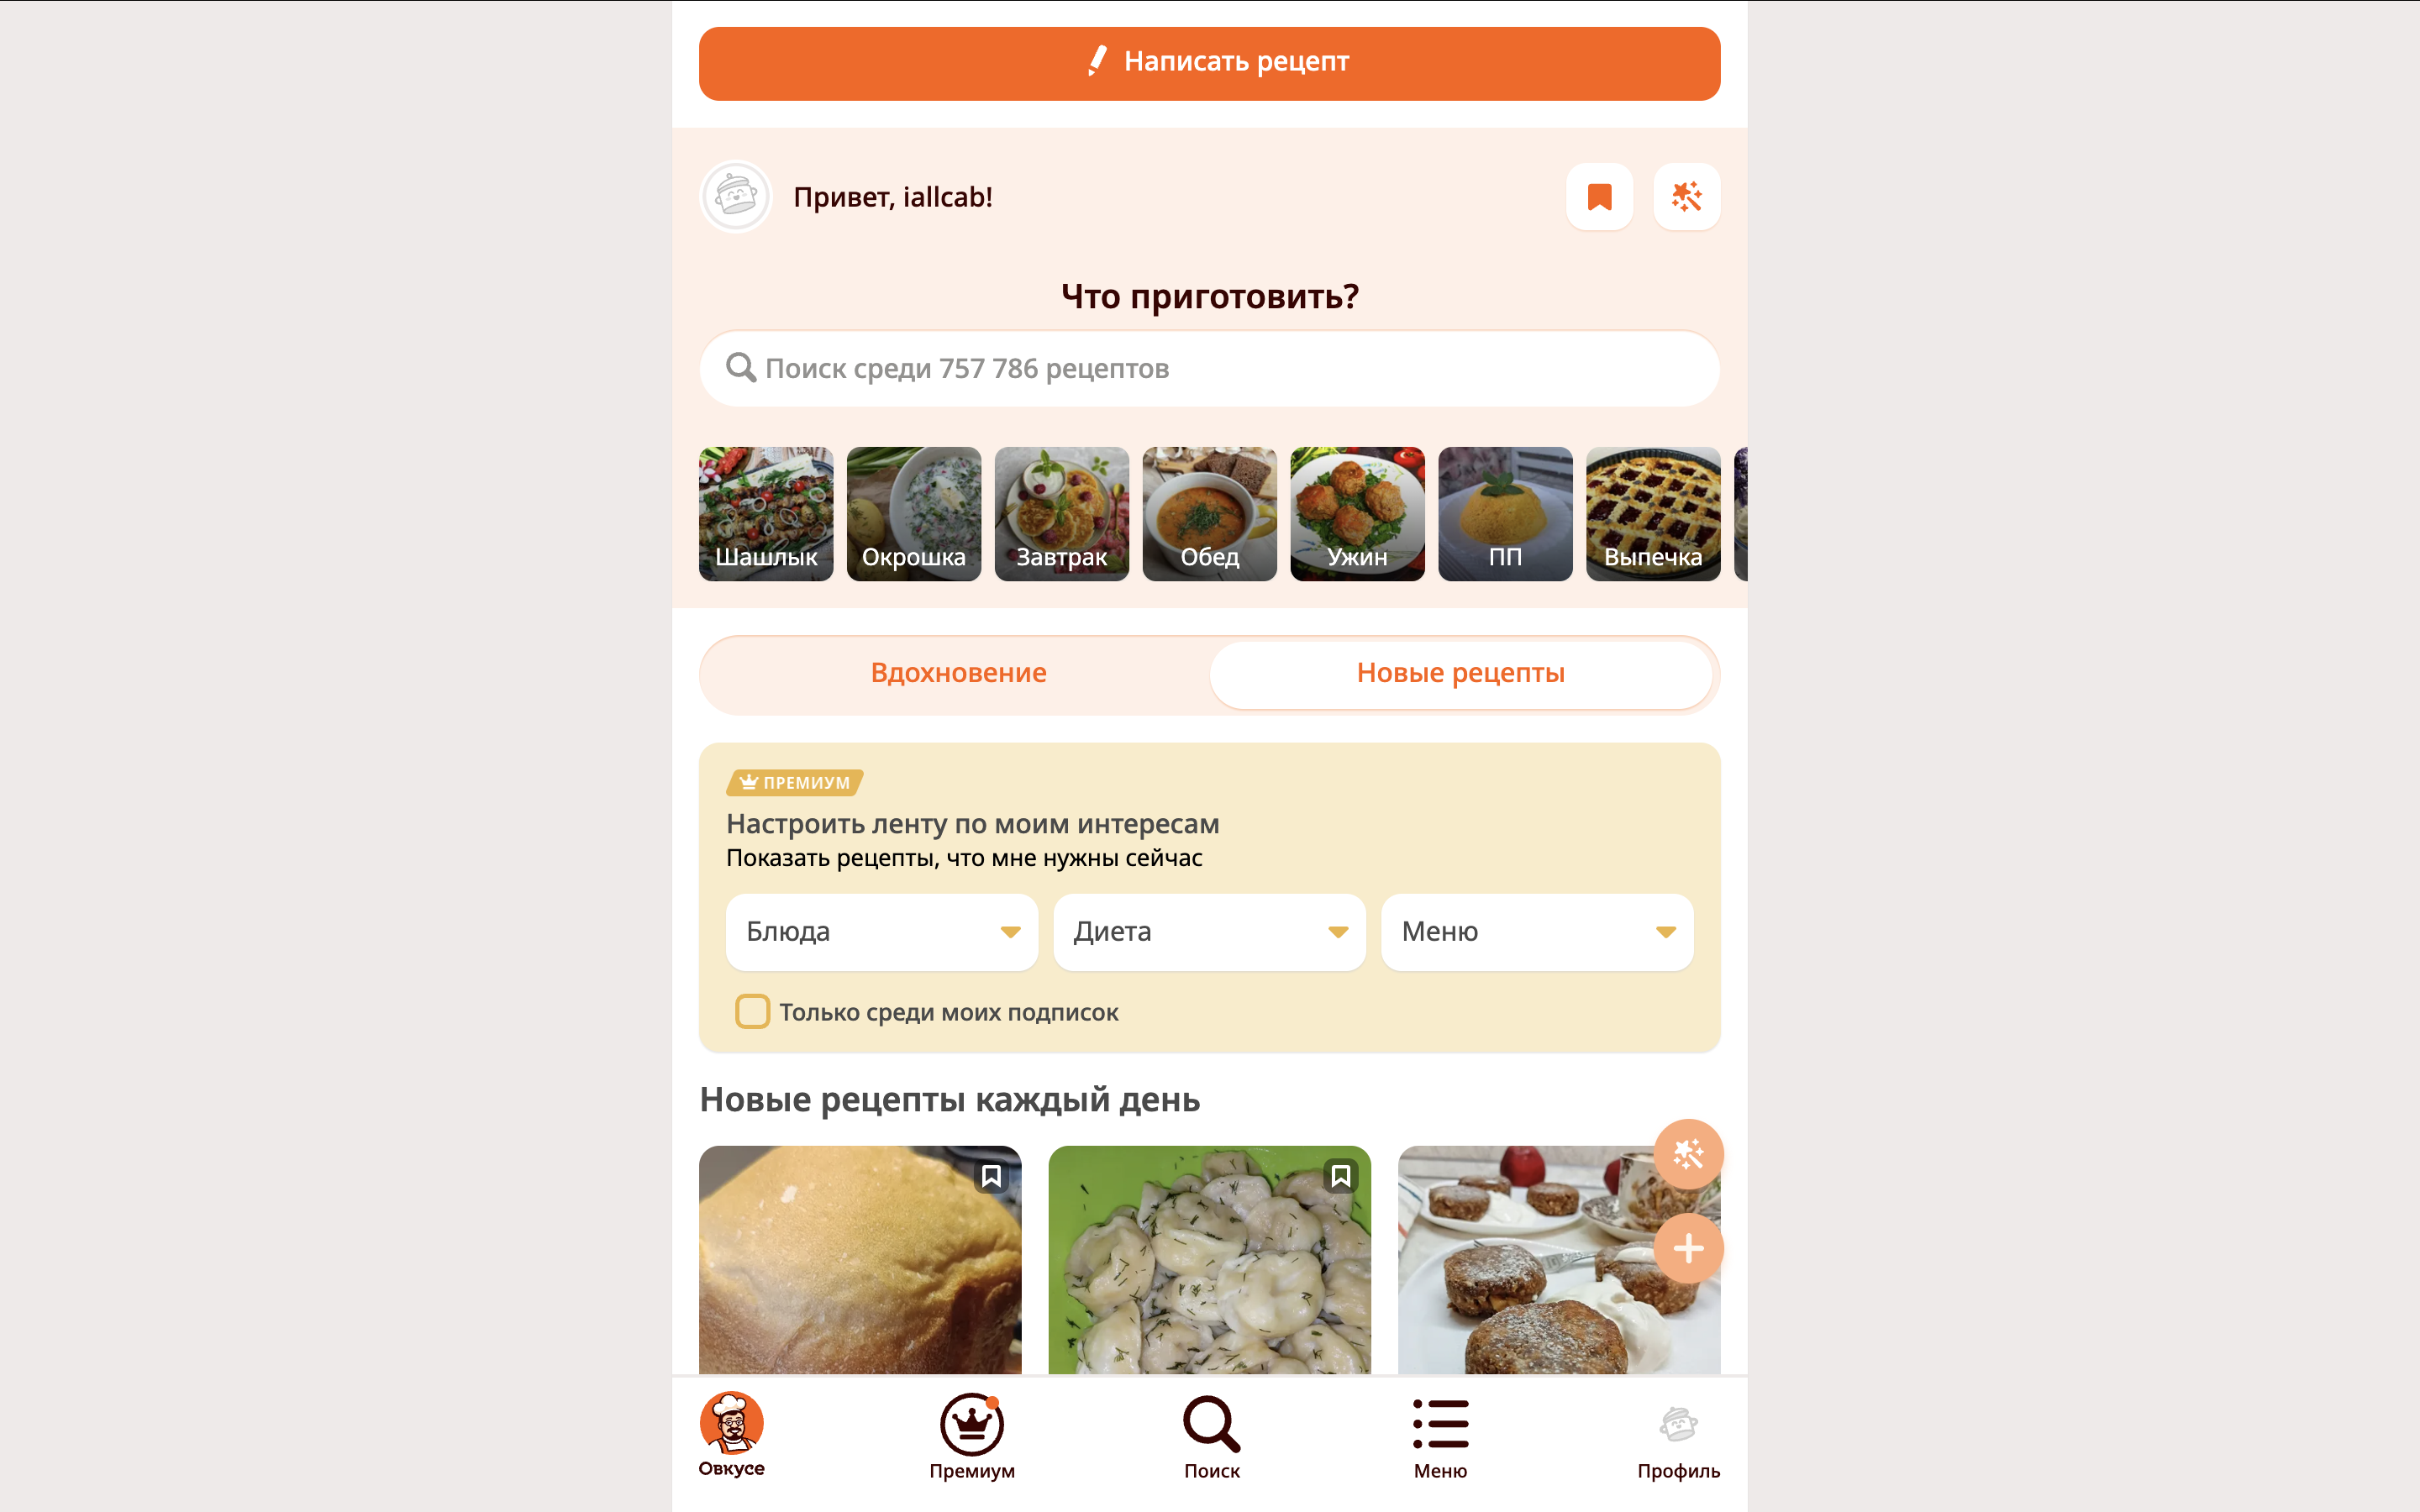
\includegraphics[width=\textwidth,height=0.82\textheight,keepaspectratio]{images/competitor-ovkuse.png}
  }{
    \fbox{\parbox{0.92\textwidth}{\centering Файл скриншота не найден: \texttt{images/competitor-ovkuse.png}}}
  }
  \caption{Интерфейс платформы Ovkuse}
  \label{fig:competitor-ovkuse}
\end{figure}

<<Поварёнок>> \cite{povarenok2026} остается сильным конкурентом как крупная кулинарная социальная платформа: в системе представлены рецепты, дневники пользователей, вопросы-ответы, статьи, посты и видеоконтент. Такой формат обеспечивает высокую активность сообщества и большой объем пользовательского контента. Одновременно интерфейс сервиса воспринимается как менее современный по сравнению с новыми продуктами, а ключевые функции FoodPlanner (конструктор плана питания и ИИ-помощник) не реализованы. Интерфейс платформы <<Поварёнок>> представлен на рисунке~\ref{fig:competitor-povarenok}.

\begin{figure}[H]
  \centering
  \IfFileExists{images/competitor-povarenok.png}{
    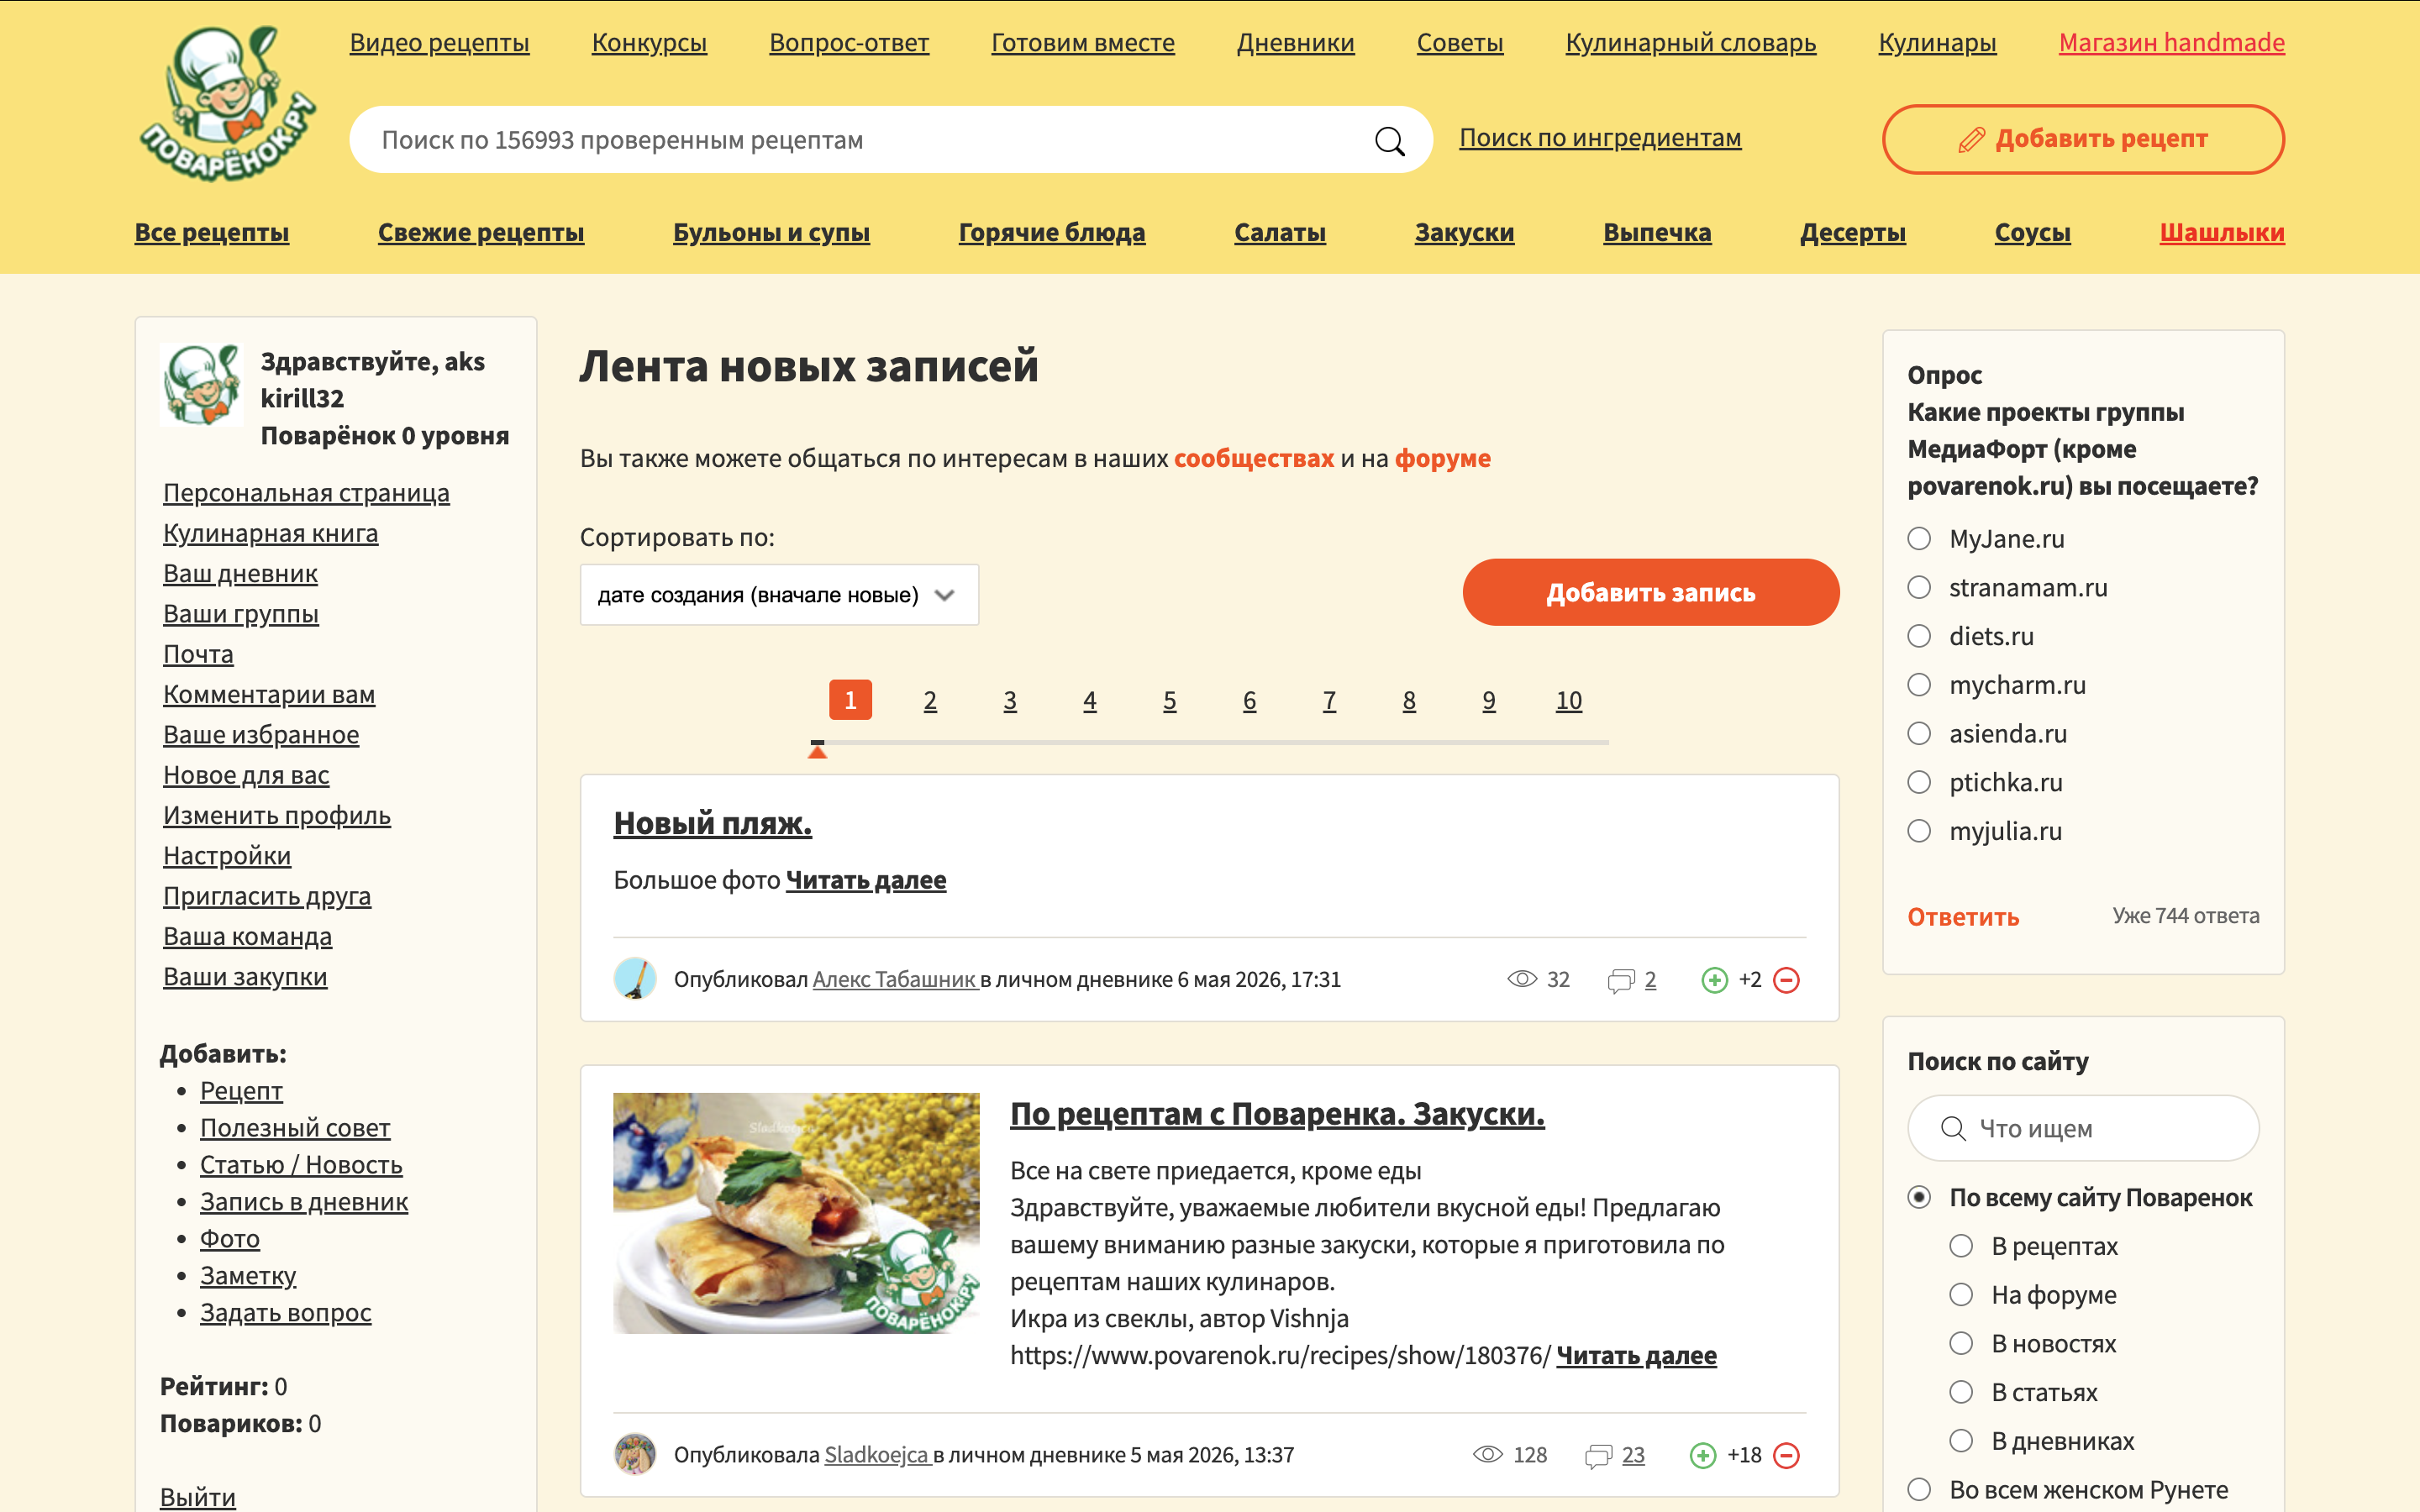
\includegraphics[width=\textwidth,height=0.82\textheight,keepaspectratio]{images/competitor-povarenok.png}
  }{
    \fbox{\parbox{0.92\textwidth}{\centering Файл скриншота не найден: \texttt{images/competitor-povarenok.png}}}
  }
  \caption{Интерфейс платформы Поварёнок}
  \label{fig:competitor-povarenok}
\end{figure}

MyFitnessPal \cite{myfitnesspal2026} задает высокий стандарт в области постановки целей и трекинга прогресса: при регистрации пользователю предлагается уточнить цель, мотивацию и параметры достижения, после чего доступны дневник питания и аналитические дэшборды. Платформа особенно сильна в фитнес- и weight-management сценариях, где важна регулярная фиксация показателей и динамики. Однако сервис в меньшей степени ориентирован на детализированное конструирование меню по дням и приемам пищи, а встроенный ИИ-ассистент отсутствует. Интерфейс платформы MyFitnessPal представлен на рисунке~\ref{fig:competitor-myfitnesspal}.

\begin{figure}[H]
  \centering
  \IfFileExists{images/competitor-myfitnesspal.png}{
    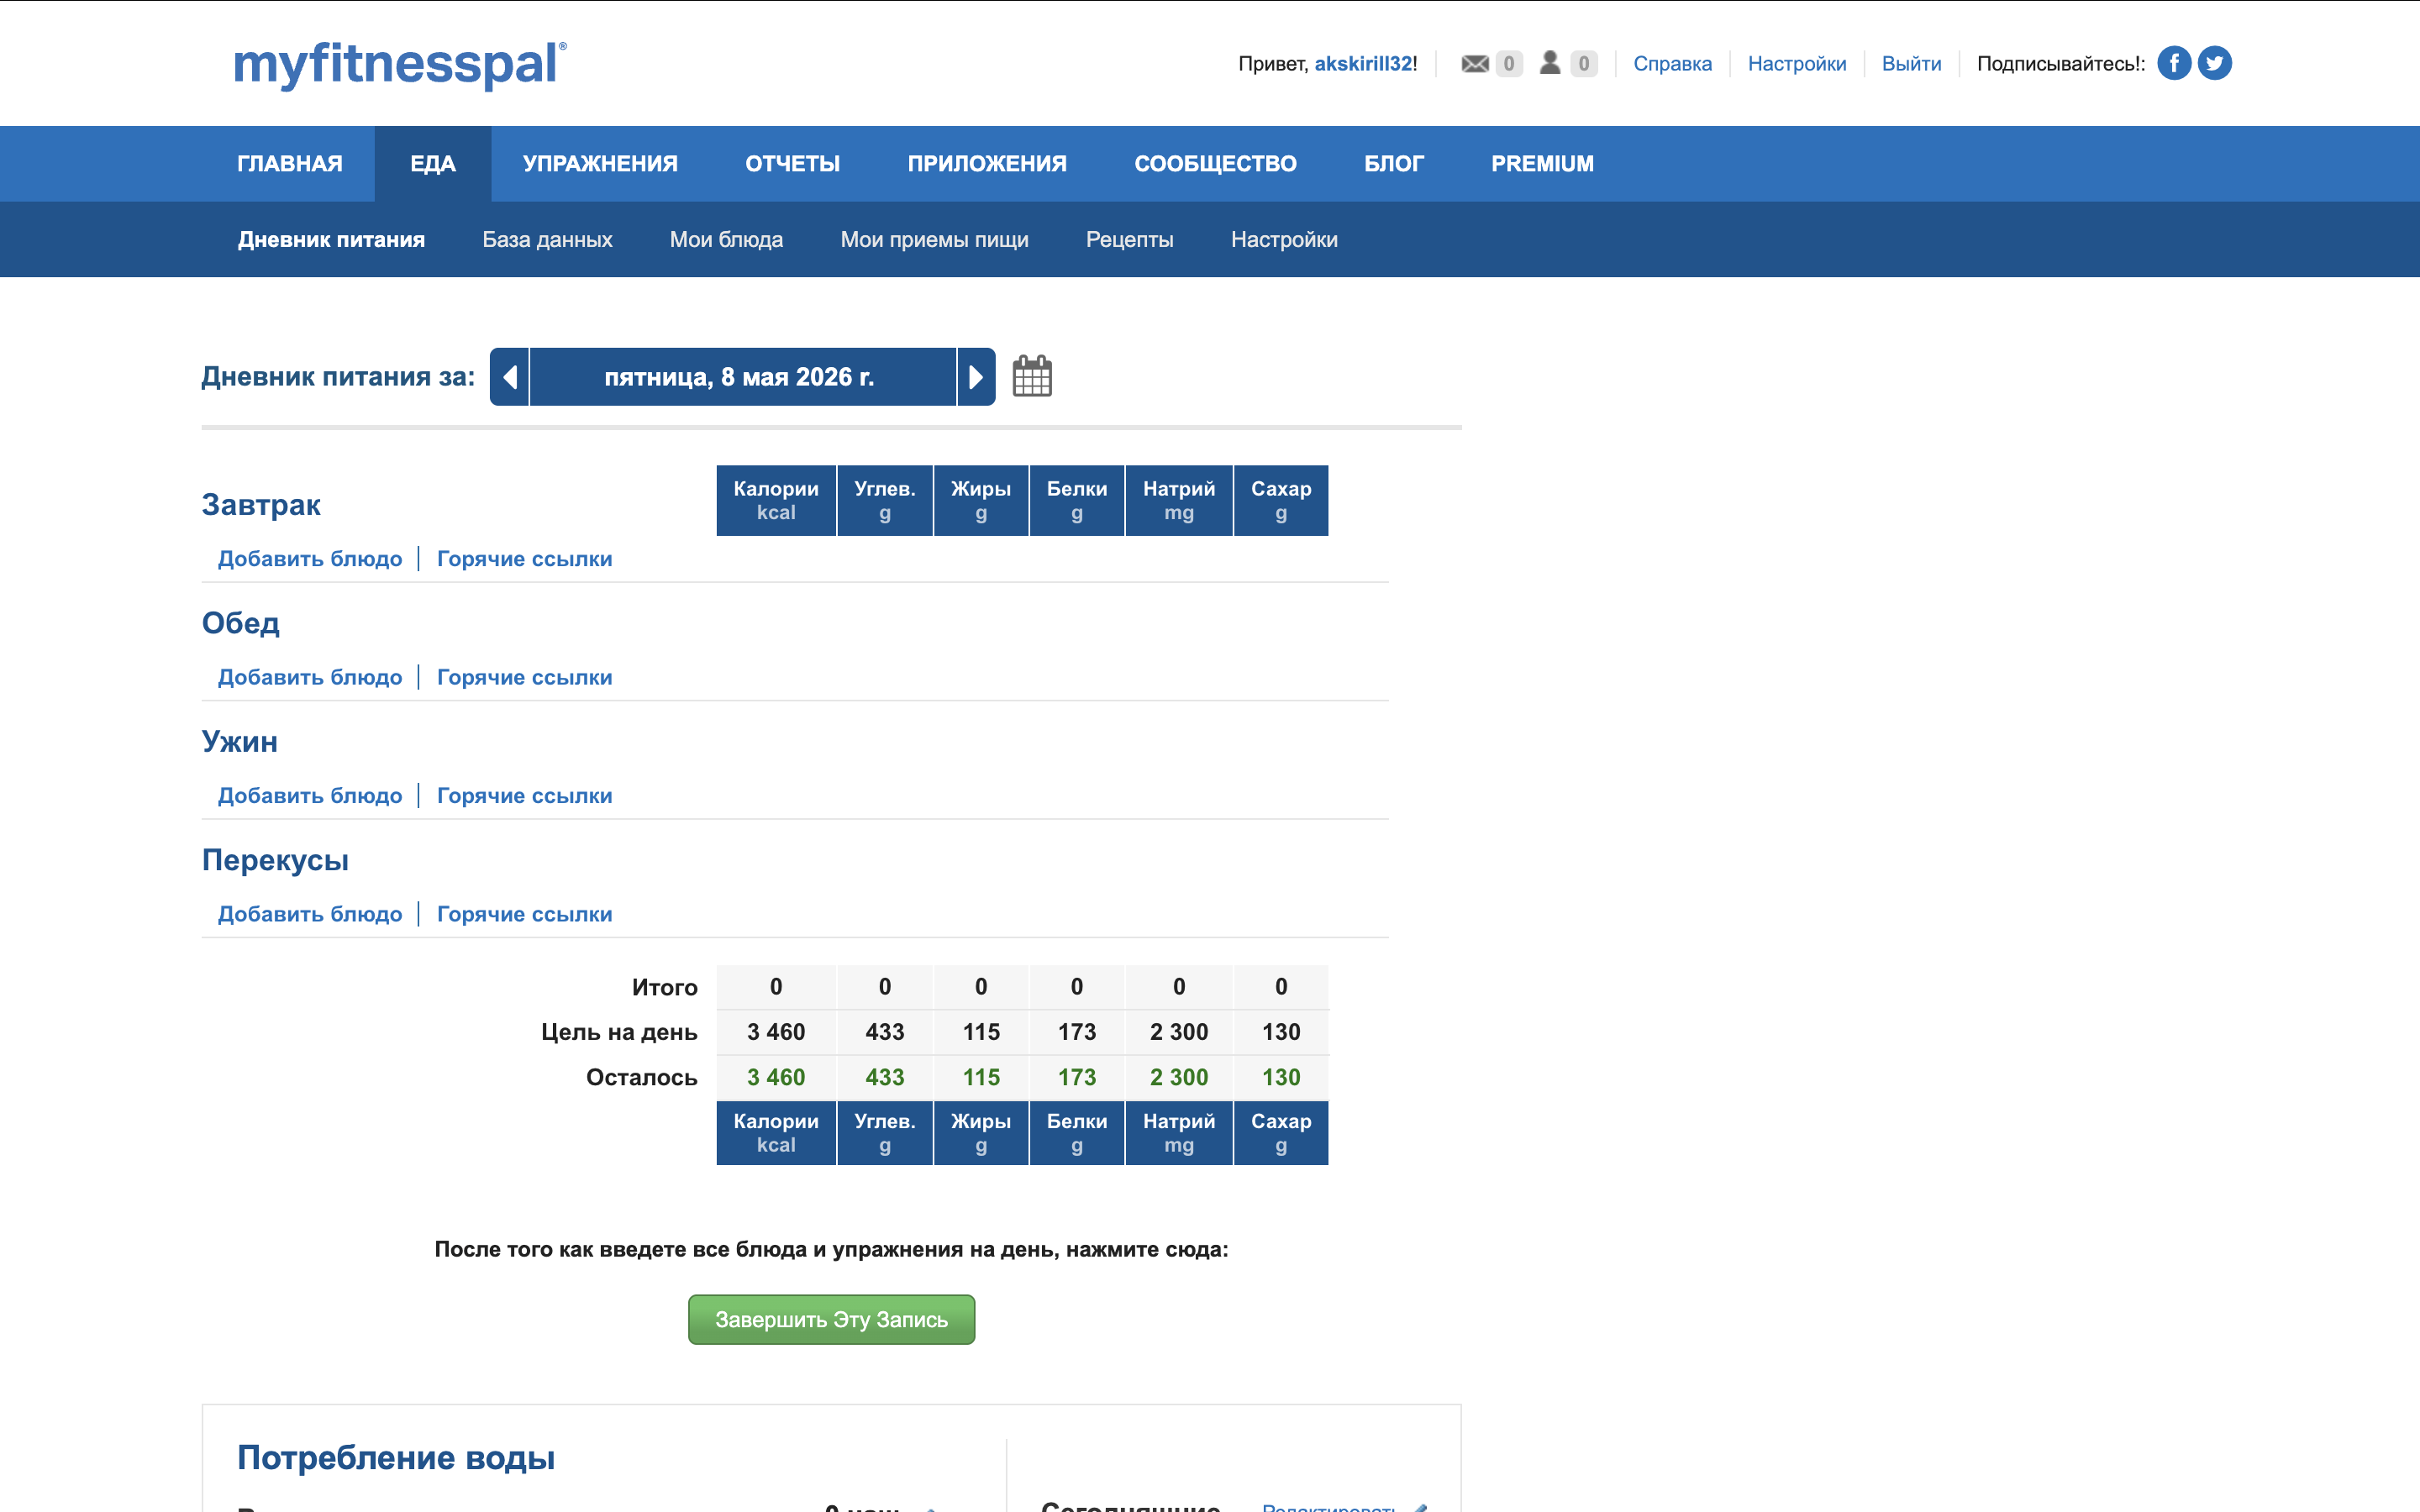
\includegraphics[width=\textwidth,height=0.82\textheight,keepaspectratio]{images/competitor-myfitnesspal.png}
  }{
    \fbox{\parbox{0.92\textwidth}{\centering Файл скриншота не найден: \texttt{images/competitor-myfitnesspal.png}}}
  }
  \caption{Интерфейс платформы MyFitnessPal}
  \label{fig:competitor-myfitnesspal}
\end{figure}

Проведенный анализ показывает, что конкуренты хорошо закрывают отдельные сегменты: контент и рецептуры, учет КБЖУ, мотивацию, социальные механики или частичную автоматизацию. При этом ни одно из рассмотренных решений не объединяет в едином контуре все целевые функции FoodPlanner: персонализированный конструктор плана питания, адаптацию под предпочтения пользователя, ИИ-сопровождение, списки покупок и ролевую модерацию контента.

\section{Определение требований к системе}

В данном разделе требования к системе представлены в порядке бизнес-приоритета: бизнес-требования, бизнес-правила и функциональные требования.

Бизнес-требования

Бизнес-требования сформулированы в измеримом виде (базовое значение~$\rightarrow$~целевое значение за 6 месяцев после запуска):
\begin{compactlist}
  \item удержание пользователей D30: 18\%~$\rightarrow$~30\%;
  \item конверсия из просмотра каталога в создание плана питания: 12\%~$\rightarrow$~25\%;
  \item доля пользователей, формирующих список покупок после создания плана: 20\%~$\rightarrow$~40\%;
  \item среднее время модерации пользовательского контента: 72~ч~$\rightarrow$~24~ч;
  \item доля жалоб, обработанных в пределах SLA 48~ч: 60\%~$\rightarrow$~90\%;
  \item доля контента с прозрачным отображением статуса модерации: 70\%~$\rightarrow$~100\%.
\end{compactlist}

Бизнес-правила

Бизнес-правила задают обязательные ограничения на поведение системы:
\begin{compactlist}
  \item ролевая модель обязательна: действия модерации доступны только ролям moderator и admin;
  \item жизненный цикл пользовательского контента фиксирован: \texttt{draft~$\rightarrow$~pending~$\rightarrow$~approved/rejected};
  \item пользователь может редактировать и удалять только собственный контент; администратор имеет расширенные права;
  \item при заполненном профиле предпочтений система обязана учитывать его в персонализированной выдаче;
  \item список покупок сохраняется с привязкой к источнику (рецепт или план питания) и доступен для повторного использования;
  \item изменения статусов модерации и ответы по жалобам сопровождаются созданием уведомлений;
  \item ключевые действия в процессах модерации и администрирования подлежат журналированию в аудите.
\end{compactlist}

Функциональные требования

Для реализации бизнес-целей выделены ключевые подсистемы, представленные в таблице~\ref{tab:subsystems-fp}.

\begin{table}[H]
\caption{Ключевые подсистемы FoodPlanner для реализации функциональных требований}
\label{tab:subsystems-fp}
\small
\begin{tabularx}{\textwidth}{|p{0.30\textwidth}|X|}
\hline
\multicolumn{1}{|c|}{Название подсистемы} & \multicolumn{1}{c|}{Описание} \\ \hline
Система управления аккаунтами и доступом & Регистрация, авторизация, управление профилем и ролевым доступом. \\ \hline
Система каталога и персонализации & Просмотр рецептов и планов, поиск, фильтрация и персонализированная выдача. \\ \hline
Система конструктора плана питания & Формирование меню по дням и приемам пищи, настройка параметров, отправка на модерацию. \\ \hline
Система модерации и обратной связи & Модерация рецептов, планов и отзывов, обработка жалоб, фиксация решений. \\ \hline
Система избранного и списков покупок & Сохранение рецептов/планов в избранное, формирование и хранение списков покупок. \\ \hline
Система уведомлений и ИИ-ассистента & Уведомления о событиях платформы и диалоговый интерфейс рекомендаций. \\ \hline
\end{tabularx}
\normalsize
\end{table}

На основании указанных подсистем сформулированы следующие функциональные требования:
\begin{compactlist}
  \item пользователь может зарегистрироваться в системе и выполнить вход по учетным данным;
  \item пользователь может просматривать и редактировать профиль (имя, фото, цели, особенности питания, теги);
  \item система поддерживает ролевую модель \texttt{user/moderator/admin} с разграничением прав;
  \item пользователь может просматривать каталоги рецептов и планов питания с поиском, фильтрацией и пагинацией;
  \item пользователь может создавать план питания в конструкторе и отправлять его на модерацию;
  \item модератор/администратор может принимать решения по модерации контента;
  \item пользователь может оставлять оценки и отзывы для рецептов и планов питания;
  \item пользователь может формировать и сохранять списки покупок с привязкой к рецепту или плану;
  \item система отображает уведомления о результатах операций и статусах модерации;
  \item пользователь может получать рекомендации через встроенный ИИ-ассистент.
\end{compactlist}

Нефункциональные требования

Ключевые нефункциональные требования:
\begin{compactlist}
  \item доступность сервиса в production: не ниже 99.5\% в месяц;
  \item медианное время ответа API для типовых запросов каталога: не более 500~мс;
  \item время загрузки ключевых страниц интерфейса при стандартном канале: не более 2~с;
  \item масштабируемость базы данных и API при росте объема данных не менее чем в 10 раз;
  \item безопасность: CSRF, ограничение CORS, хэширование паролей, HTTPS, отсутствие ключей внешних API на клиенте \cite{owasp_top10_2021,owasp_csrf_cheatsheet,owasp_xss_cheatsheet,owasp_sqli_cheatsheet,django_cors_headers_docs_2026};
  \item сопровождаемость: модульная структура frontend/backend и документированные контракты API.
\end{compactlist}

\section{Проектирование архитектуры системы}

Общая структура данных в приложении

Общая структура данных и потоков в FoodPlanner может быть формализована через DFD-представление. Контекстная диаграмма отражает взаимодействие системы с ключевыми внешними сущностями:
\begin{compactlist}
  \item пользователь платформы (формирование рациона, работа с рецептами и планами);
  \item модератор и администратор (контроль качества контента и управление системой);
  \item клиентское веб-приложение (SPA), выступающее основным каналом пользовательского взаимодействия;
  \item внешние сервисы (например, API ИИ-ассистента).
\end{compactlist}

Контекстная DFD-диаграмма представлена на рисунке~\ref{fig:dfd-context}.

\begin{figure}[H]
  \centering
  \IfFileExists{images/dfd-context.png}{
    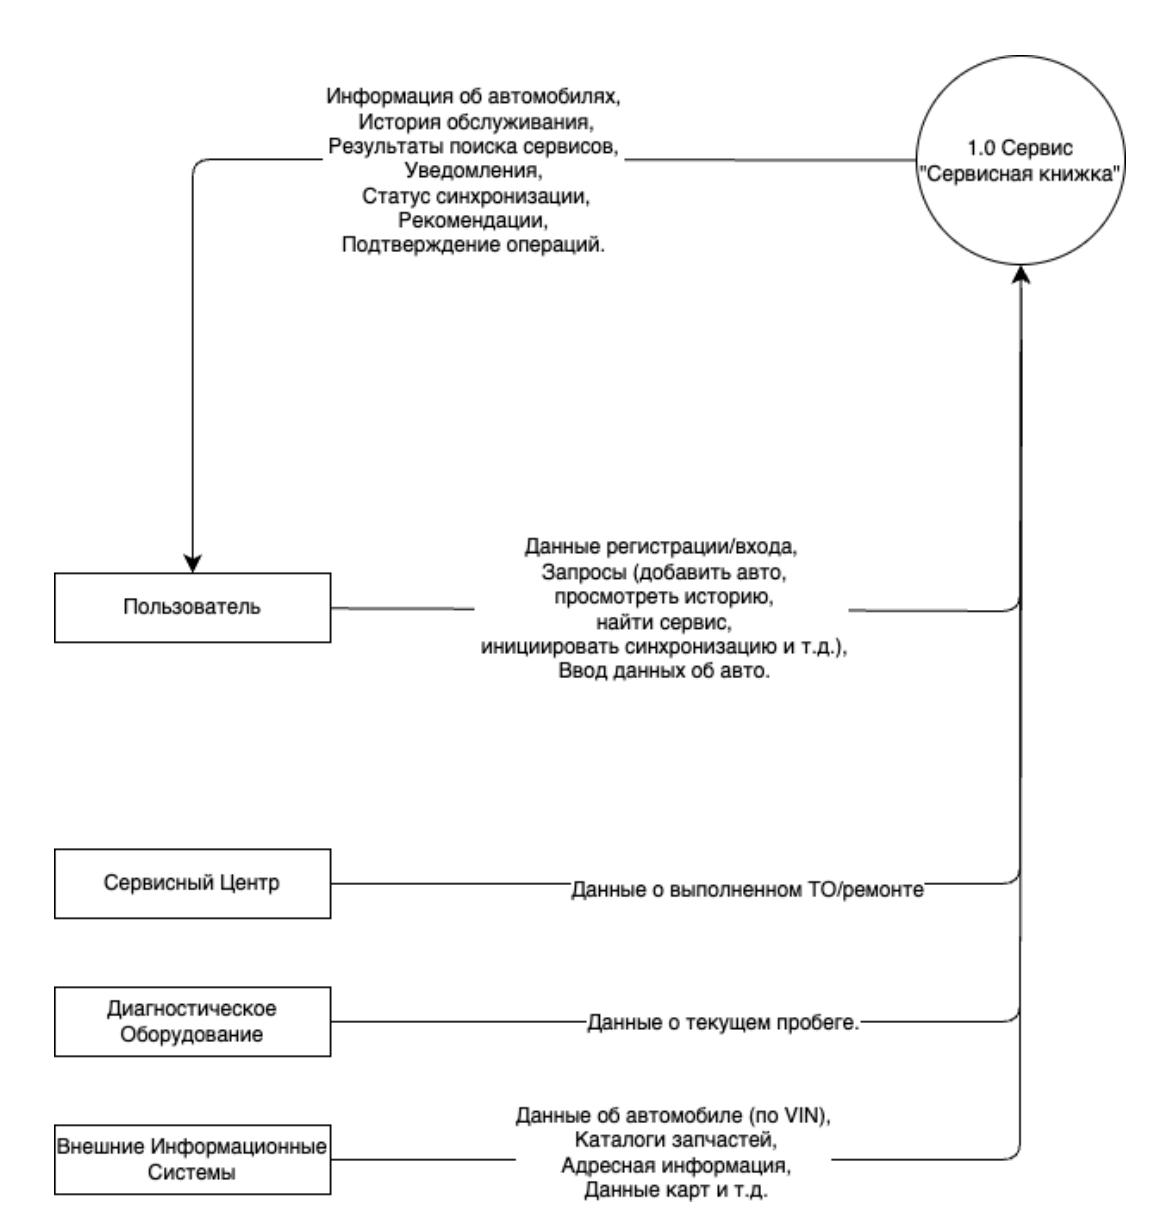
\includegraphics[width=\textwidth,height=0.82\textheight,keepaspectratio]{dfd-context.png}
  }{
    \fbox{\parbox{0.9\textwidth}{\centering Место для контекстной DFD-диаграммы\\
    Файл: \texttt{Report/images/dfd-context.png}}}
  }
  \caption{Контекстная DFD-диаграмма FoodPlanner}
  \label{fig:dfd-context}
\end{figure}

При детализации DFD-уровня выделяются основные процессы и хранилища данных.

Процессы:
\begin{compactlist}
  \item управление пользователями и аутентификацией;
  \item управление рецептами, тегами, категориями и ингредиентами;
  \item управление планами питания и генерацией списков покупок;
  \item модерация пользовательского контента и обработка жалоб;
  \item управление отзывами, избранным и уведомлениями;
  \item взаимодействие с внешним API ИИ-ассистента.
\end{compactlist}

Хранилища данных:
\begin{compactlist}
  \item DS1: учетные записи, роли и настройки профилей пользователей;
  \item DS2: рецепты, планы питания, структура рационов и shopping list;
  \item DS3: отзывы, жалобы, модерационные журналы и уведомления.
\end{compactlist}

Детализированная DFD-диаграмма представлена на рисунке~\ref{fig:dfd-level1}.

\begin{figure}[H]
  \centering
  \IfFileExists{images/dfd-level1.png}{
    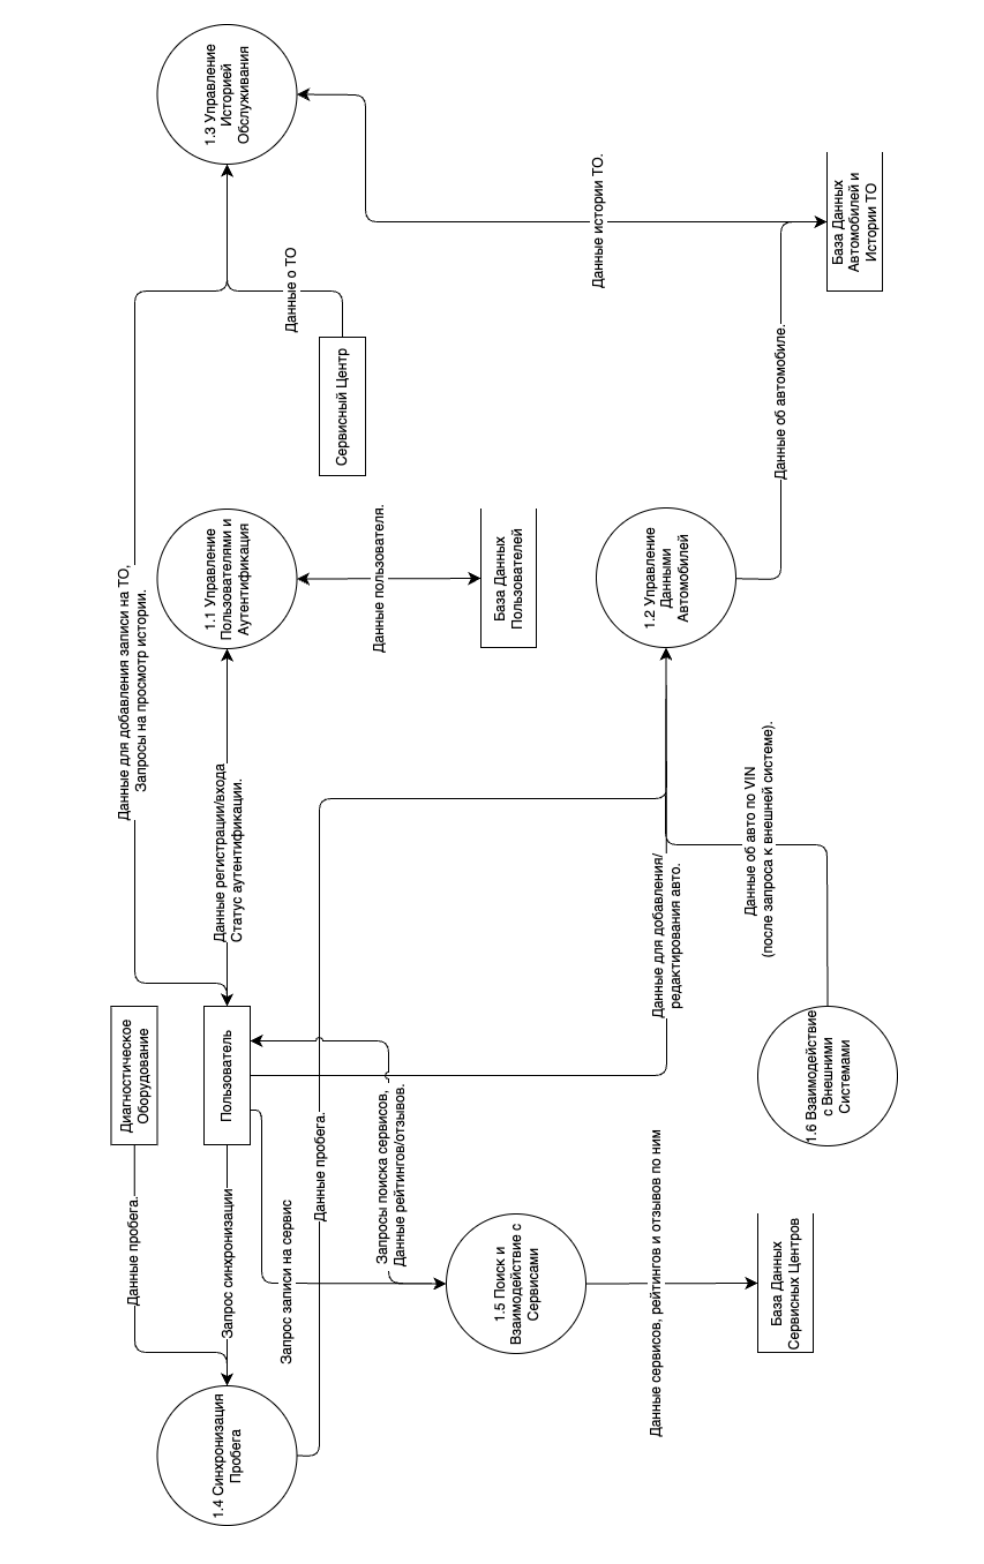
\includegraphics[width=\textwidth,height=0.82\textheight,keepaspectratio]{dfd-level1.png}
  }{
    \fbox{\parbox{0.9\textwidth}{\centering Место для детализированной DFD-диаграммы\\
    Файл: \texttt{Report/images/dfd-level1.png}}}
  }
  \caption{DFD-диаграмма процессов и хранилищ данных FoodPlanner}
  \label{fig:dfd-level1}
\end{figure}

Такая организация данных и потоков обеспечивает целостность информации и упрощает масштабирование системы при росте количества пользователей и контента.

Выбор архитектуры веб-сервиса

Для FoodPlanner выбрана клиент-серверная архитектура: клиентская часть (React + TypeScript) и серверная часть (Django + DRF) реализованы как независимые модули с единым API-контрактом. Альтернативным вариантом могла быть микросервисная архитектура, однако для текущего масштаба проекта и размера команды она избыточна по операционной сложности.

Схематичное представление клиент-серверной архитектуры и микросервисного подхода показано на рисунках~\ref{fig:arch-client-server} и~\ref{fig:arch-microservices}.

\begin{figure}[H]
  \centering
  \IfFileExists{images/arch-client-server.png}{
    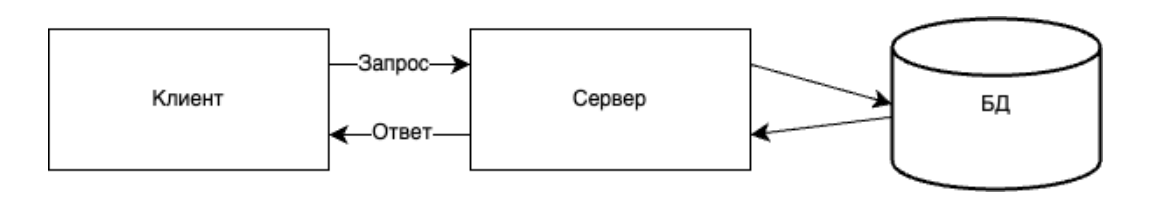
\includegraphics[width=\textwidth,height=0.82\textheight,keepaspectratio]{arch-client-server.png}
  }{
    \fbox{\parbox{0.9\textwidth}{\centering Место для схемы клиент-серверной архитектуры\\
    Файл: \texttt{Report/images/arch-client-server.png}}}
  }
  \caption{Клиент-серверная архитектура FoodPlanner}
  \label{fig:arch-client-server}
\end{figure}

\begin{figure}[H]
  \centering
  \IfFileExists{images/arch-microservices.png}{
    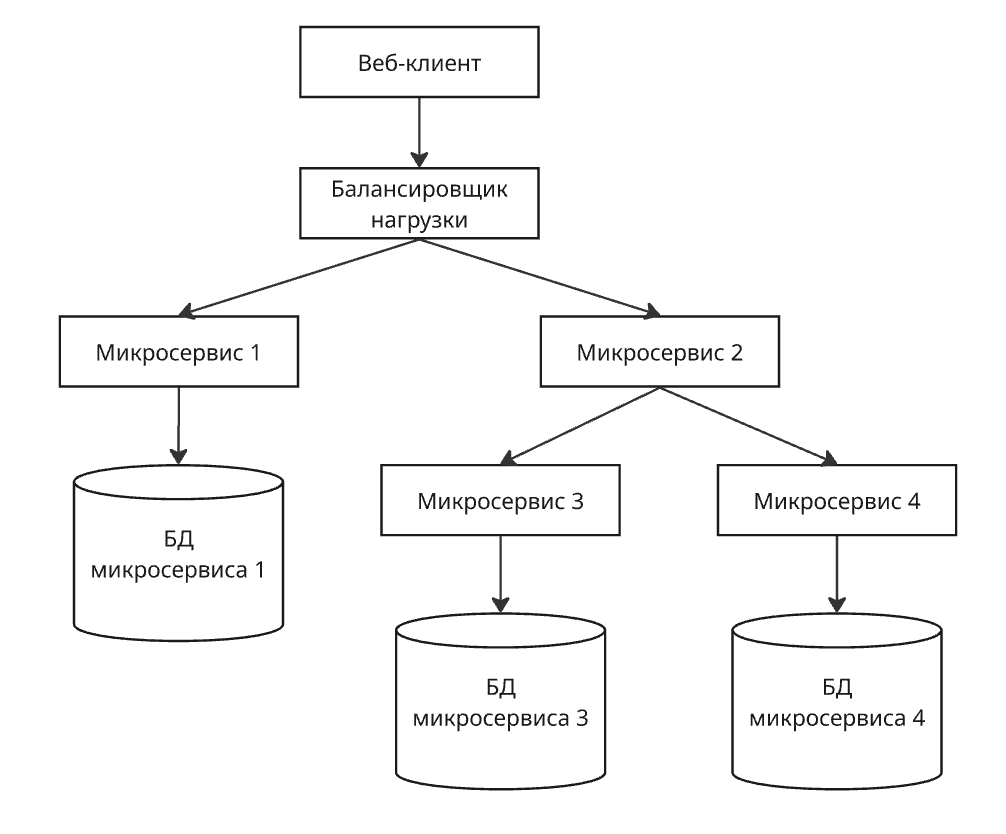
\includegraphics[width=\textwidth,height=0.82\textheight,keepaspectratio]{arch-microservices.png}
  }{
    \fbox{\parbox{0.9\textwidth}{\centering Место для схемы микросервисной архитектуры\\
    Файл: \texttt{Report/images/arch-microservices.png}}}
  }
  \caption{Микросервисная архитектура (альтернативный подход)}
  \label{fig:arch-microservices}
\end{figure}

Сравнительный анализ клиент-серверной и микросервисной архитектур приведен в таблице~\ref{tab:arch-compare}.

\begin{table}[H]
\caption{Сравнение клиент-серверной и микросервисной архитектур}
\label{tab:arch-compare}
\small
\begin{tabularx}{\textwidth}{|p{0.21\textwidth}|p{0.36\textwidth}|X|}
\hline
\multicolumn{1}{|c|}{Критерий} & \multicolumn{1}{c|}{Клиент-серверная архитектура} & \multicolumn{1}{c|}{Микросервисная архитектура} \\ \hline
Принцип & Единый централизованный backend для обслуживания клиентов & Набор автономных сервисов, каждый отвечает за свою предметную область \\ \hline
Компоненты & SPA-клиент, API-сервер, единая БД & Набор сервисов, API-шлюз, межсервисное взаимодействие, распределенные БД \\ \hline
Масштабируемость & Масштабирование преимущественно на уровне всего backend & Независимое масштабирование отдельных сервисов \\ \hline
Развертывание & Единый релизный контур и более простой процесс деплоя & Независимые релизы, более сложная инфраструктура CI/CD \\ \hline
Сложность разработки & Ниже, проще старт и сопровождение малой командой & Выше из-за распределенности и усложнения инфраструктуры \\ \hline
Надежность при сбоях & Критические сбои затрагивают сервис целиком & Сбой одного сервиса ограниченно влияет на систему в целом \\ \hline
Коммуникация & Централизованные HTTP-запросы к одному API & HTTP/gRPC + асинхронные шины и очереди \\ \hline
Тестирование & Проще сквозное тестирование & Требуется отдельно тестировать сервисы и интеграции \\ \hline
\end{tabularx}
\normalsize
\end{table}

Для текущих требований FoodPlanner, объема команды и ресурсов клиент-серверная архитектура обеспечивает оптимальный баланс между скоростью разработки и эксплуатационной устойчивостью, сохраняя возможность дальнейшего масштабирования.

Для дальнейшей детализации архитектуры используется C4-подход, разделяющий описание системы на уровни абстракции:
\begin{compactlist}
  \item Context --- система в окружении пользователей и внешних сервисов;
  \item Container --- клиент, backend, база данных и внешние интеграции;
  \item Component --- внутренние модули backend и frontend по доменным областям;
  \item Code --- уровень классов/модулей и программной реализации.
\end{compactlist}

Проектирование базы данных

При выборе модели хранения данных для FoodPlanner рассматривались основные типы баз данных:
\begin{compactlist}
  \item реляционные БД --- строгая схема, SQL, ACID-транзакции, высокая целостность;
  \item документо-ориентированные БД --- гибкая схема и высокая адаптивность форматов;
  \item key-value и колоночные БД --- высокая производительность в специализированных сценариях.
\end{compactlist}

Сравнительная характеристика моделей данных представлена в таблице~\ref{tab:db-model-compare}.

\begin{table}[H]
\caption{Сравнительная характеристика моделей баз данных}
\label{tab:db-model-compare}
\small
\begin{tabularx}{\textwidth}{|p{0.22\textwidth}|p{0.24\textwidth}|X|}
\hline
\multicolumn{1}{|c|}{Критерий} & \multicolumn{1}{c|}{Реляционная модель} & \multicolumn{1}{c|}{Гибкие NoSQL-модели} \\ \hline
Структура данных & Таблицы, связи, строгая схема & Документы/ключ-значение/колонки, схема гибкая \\ \hline
Целостность & Высокая за счет ограничений и внешних ключей & Часто контролируется на уровне приложения \\ \hline
Транзакционность & Полная поддержка ACID & Поддержка зависит от конкретной СУБД \\ \hline
Язык запросов & Стандартизированный SQL & Специфичные API и языки запросов \\ \hline
Оптимальный сценарий & Бизнес-системы с богатой связностью данных и требованиями целостности & Высоконагруженные узкоспециализированные сценарии \\ \hline
\end{tabularx}
\normalsize
\end{table}

Для FoodPlanner выбрана реляционная модель с использованием PostgreSQL, так как система оперирует связанной доменной моделью (пользователи, рецепты, планы, отзывы, жалобы, уведомления), для которой критичны целостность, предсказуемость запросов и транзакционная согласованность.

Логическая схема данных отражает ключевые сущности предметной области и связи между ними. Центральными таблицами являются \texttt{users}, \texttt{recipes}, \texttt{ingredients}, \texttt{meal\_plans}, \texttt{reviews}, \texttt{complaints}, \texttt{favorites}, \texttt{notifications}, а также связующие таблицы \texttt{recipe\_ingredients}, \texttt{meal\_plan\_items}, \texttt{shopping\_list\_items}.

Внешние ключи, ограничения уникальности и индексы обеспечивают корректность и производительность типовых пользовательских запросов.

Ключевые элементы логической модели представлены ниже фрагментами реальной серверной реализации.

\begin{listing}[H]
\caption{Модель ролей и пользователей}
\label{listing:user-role-model}
\begin{mdframed}
\begin{minted}[breaklines=true]{python}
class Role(models.Model):
    class RoleNames(models.TextChoices):
        USER = "user", "User"
        MODERATOR = "moderator", "Moderator"
        ADMIN = "admin", "Admin"

    name = models.CharField(max_length=32, unique=True, choices=RoleNames.choices)

class User(AbstractUser):
    username = None
    email = models.EmailField(unique=True)
    role = models.ForeignKey(Role, on_delete=models.SET_NULL, null=True, blank=True)
    health_features = models.JSONField(default=list, blank=True)
    favorite_tags = models.JSONField(default=list, blank=True)
    USERNAME_FIELD = "email"
\end{minted}
\end{mdframed}
\end{listing}

\begin{listing}[H]
\caption{Фрагмент модели рецептов и состава ингредиентов}
\label{listing:recipe-model}
\begin{mdframed}
\begin{minted}[breaklines=true]{python}
class Recipe(models.Model):
    title = models.CharField(max_length=255)
    category = models.ForeignKey(Category, on_delete=models.SET_NULL, null=True, blank=True)
    author = models.ForeignKey(settings.AUTH_USER_MODEL, on_delete=models.CASCADE)
    status = models.CharField(max_length=16, choices=ModerationStatus.choices)
    tags = models.ManyToManyField(Tag, related_name="recipes", blank=True)

    class Meta:
        indexes = [
            models.Index(fields=["author"]),
            models.Index(fields=["category"]),
            models.Index(fields=["status"]),
        ]

class RecipeIngredient(models.Model):
    recipe = models.ForeignKey(Recipe, on_delete=models.CASCADE, related_name="recipe_ingredients")
    ingredient = models.ForeignKey(Ingredient, on_delete=models.CASCADE)
    quantity = models.DecimalField(max_digits=10, decimal_places=2)
\end{minted}
\end{mdframed}
\end{listing}

\begin{listing}[H]
\caption{Фрагмент модели плана питания и списка покупок}
\label{listing:mealplan-shopping-model}
\begin{mdframed}
\begin{minted}[breaklines=true]{python}
class MealPlan(models.Model):
    user = models.ForeignKey(settings.AUTH_USER_MODEL, on_delete=models.CASCADE)
    start_date = models.DateField()
    end_date = models.DateField()
    status = models.CharField(max_length=16, choices=Status.choices, default=Status.DRAFT)

class MealPlanItem(models.Model):
    meal_plan = models.ForeignKey(MealPlan, on_delete=models.CASCADE, related_name="items")
    day_number = models.PositiveSmallIntegerField()
    meal_type = models.CharField(max_length=16, choices=MealType.choices)
    recipe = models.ForeignKey("recipes.Recipe", on_delete=models.CASCADE)

class ShoppingList(models.Model):
    user = models.ForeignKey(settings.AUTH_USER_MODEL, on_delete=models.CASCADE)
    target_type = models.CharField(max_length=16, choices=TargetType.choices, blank=True, default="")
    target_id = models.PositiveBigIntegerField(null=True, blank=True)
\end{minted}
\end{mdframed}
\end{listing}

\begin{figure}[H]
  \centering
  \IfFileExists{images/data-model.png}{
    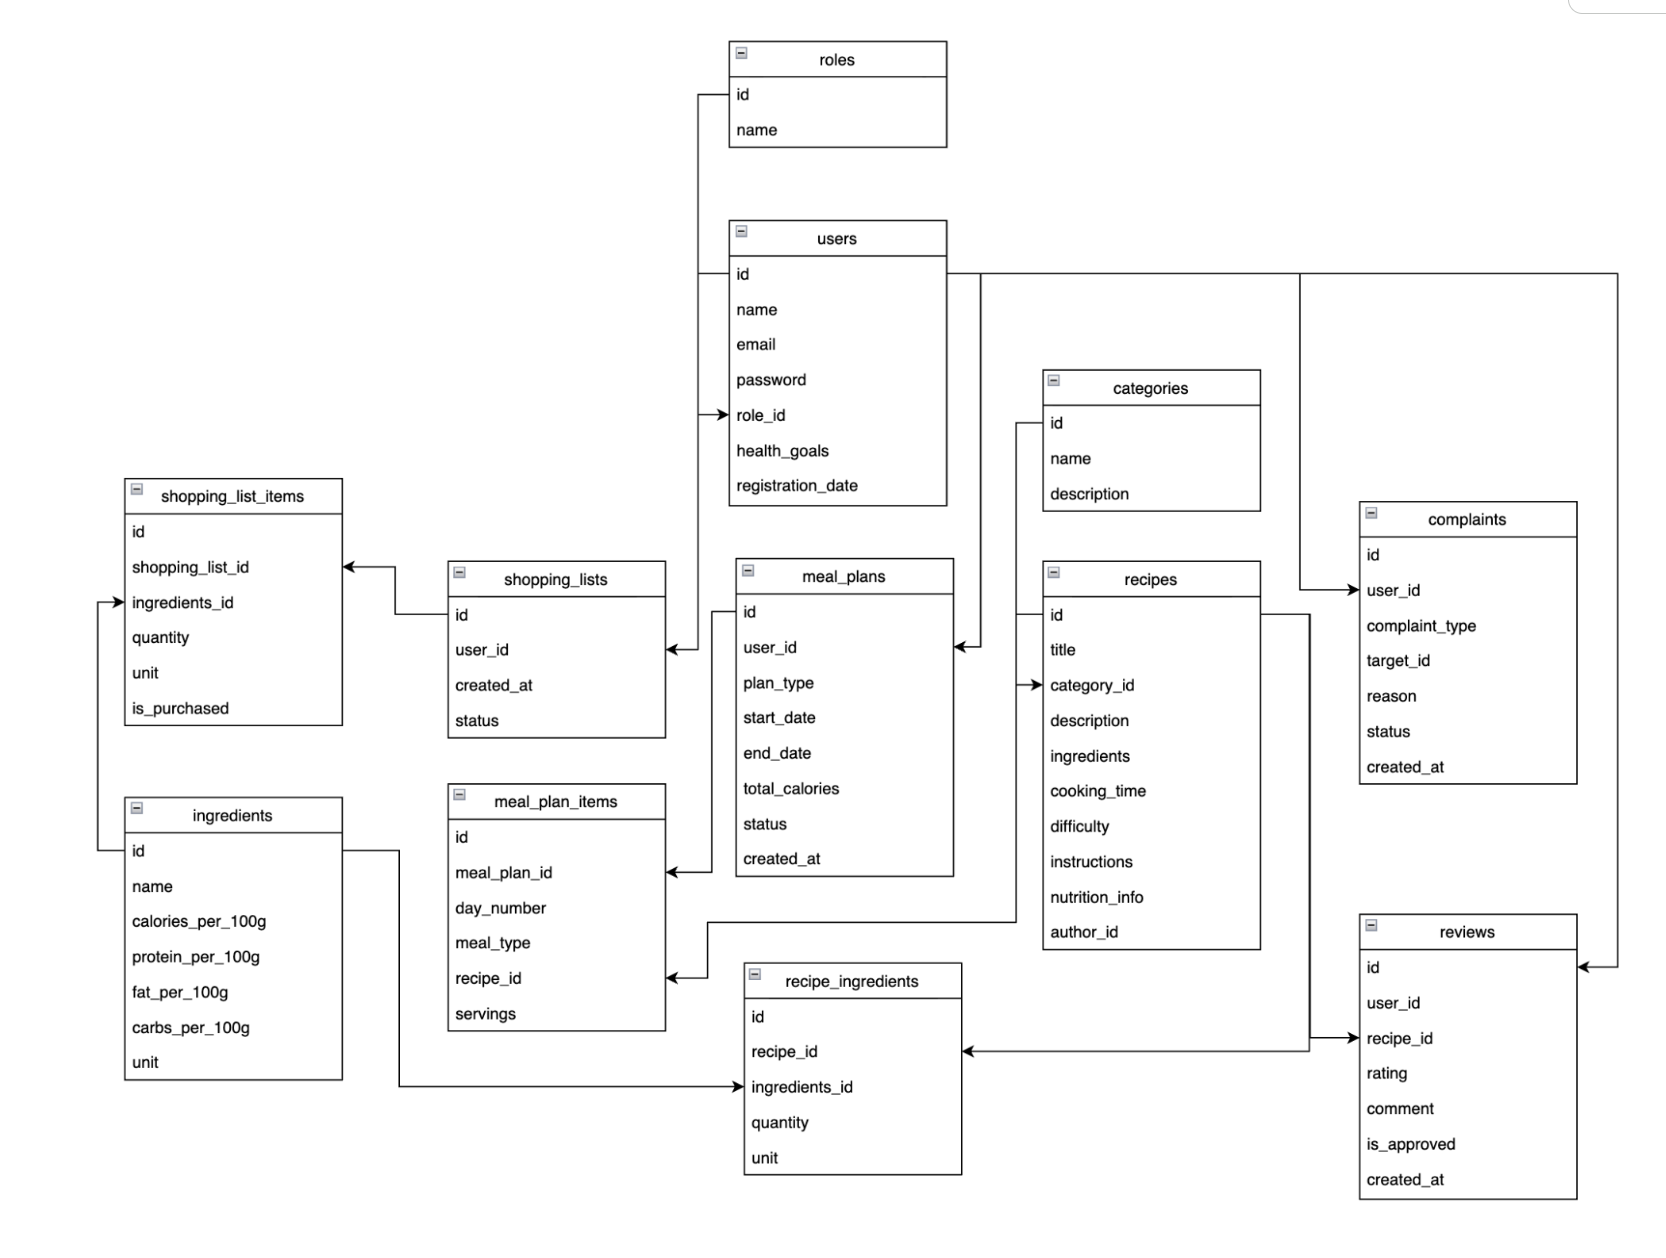
\includegraphics[width=0.95\textwidth]{data-model.png}
  }{
    \fbox{\parbox{0.9\textwidth}{\centering Место для ER-диаграммы\\
    Файл: \texttt{Report/images/data-model.png}}}
  }
  \caption{Логическая модель данных FoodPlanner}
  \label{fig:data-model}
\end{figure}

\section{Выбор программных и технических средств разработки}

Для разработки FoodPlanner использован клиент-серверный подход, поэтому технологический стек разделен на две части: клиентскую (frontend) и серверную (backend). При выборе инструментов учитывались критерии производительности, скорости разработки, удобства сопровождения, зрелости экосистемы и соответствия функциональным требованиям проекта.

Серверная часть реализована на Python с использованием Django и Django REST Framework \cite{python_docs_2026,django_docs_2026,drf_docs_2026}. В качестве СУБД выбрана PostgreSQL \cite{postgresql_docs_2026}. Для контейнеризации и воспроизводимого развертывания используется Docker и Docker Compose \cite{docker_docs_2026,docker_compose_docs_2026}.

Для клиентской части выбраны React + TypeScript, управление состоянием выполнено на Effector, UI-слой построен на Mantine, сборка и локальная разработка выполняются через Vite \cite{react_docs_2026,typescript_docs_2026,effector_docs_2026,mantine_docs_2026,vite_docs_2026}.

Сравнительный анализ серверных языков разработки для проекта приведен в таблице~\ref{tab:backend-lang-compare} с опорой на официальные материалы по языкам и платформам \cite{python_docs_2026,java_docs_2026,nodejs_docs_2026,go_docs_2026}.

\begin{table}[H]
\caption{Сравнительный анализ серверных языков}
\label{tab:backend-lang-compare}
\begin{tabularx}{\textwidth}{|p{0.16\textwidth}|p{0.38\textwidth}|X|}
\hline
\multicolumn{1}{|c|}{Язык} & \multicolumn{1}{c|}{Преимущества} & \multicolumn{1}{c|}{Ограничения для проекта} \\ \hline
Python & Высокая скорость разработки, зрелые веб-фреймворки, низкий порог вхождения & Ниже производительность в CPU-интенсивных задачах по сравнению с компилируемыми языками \\ \hline
Java & Высокая надежность и производительность, зрелая экосистема enterprise-решений & Более высокая сложность и объем кода для быстрого прототипирования \\ \hline
Node.js (TS/JS) & Единый язык для frontend/backend, высокая скорость I/O-сценариев & Требует более строгой дисциплины архитектуры в больших проектах \\ \hline
Go & Высокая производительность и эффективная конкурентность & Меньшая гибкость и более узкая экосистема для сложных административных сценариев \\ \hline
\end{tabularx}
\end{table}

Для прикладных задач FoodPlanner (быстрая реализация доменных модулей, ролевой доступ, модерация, административная логика, API-подход) выбор Python + Django признан оптимальным по балансу трудозатрат и эксплуатационной надежности.

Сравнение выбранных средств клиентской разработки приведено в таблице~\ref{tab:frontend-stack-compare}.

\begin{table}[H]
\caption{Выбор средств клиентской разработки}
\label{tab:frontend-stack-compare}
\begin{tabularx}{\textwidth}{|p{0.26\textwidth}|X|}
\hline
\multicolumn{1}{|c|}{Компонент стека} & \multicolumn{1}{c|}{Обоснование выбора} \\ \hline
React + TypeScript & Компонентный подход, типобезопасность и удобная поддержка сложных интерфейсных сценариев \\ \hline
Effector & Детерминированное управление состоянием и понятная модель асинхронных процессов \\ \hline
Mantine & Быстрое построение консистентного UI и сокращение времени реализации типовых паттернов \\ \hline
Vite & Быстрый цикл разработки и сборки SPA-приложения \\ \hline
\end{tabularx}
\end{table}

Таким образом, выбранные программные и технические средства обеспечивают покрытие функциональных требований, поддержку безопасного взаимодействия клиентской и серверной частей, а также возможность поэтапного масштабирования системы.

\section{Выводы по главе}

В первой главе определен проблемный контекст предметной области: пользователи решают взаимосвязанные задачи планирования питания в разрозненных сервисах, что приводит к фрагментации данных и избыточным трудозатратам.

На основании обзора аналогов подтверждено наличие рыночных решений с сильными сторонами, однако выявлены ограничения при реализации комплексного сценария. Это обосновывает разработку собственного веб-приложения, объединяющего полный цикл планирования рациона.

Также сформированы целевая аудитория и ролевая модель, определены функциональные, бизнес- и нефункциональные требования, проведен сравнительный анализ конкурентов и аналогов, описаны бизнес-процессы в IDEF-нотациях и зафиксирована модель данных системы.
\chapter{{\fontsize{14pt}{21pt}\selectfont\MakeUppercase{Техническая реализация системы}}}
\label{cha:design}

\section{Разработка пользовательского интерфейса приложения}

Для реализации пользовательского интерфейса веб-приложения FoodPlanner использовались React и библиотека компонентов Mantine. Выбранный технологический стек позволил сократить время разработки, обеспечить единый визуальный стиль экранов и повысить предсказуемость поведения интерфейса.

Главная страница выполняет функцию стартового навигационного узла и предоставляет пользователю структурированное представление о возможностях платформы. На странице размещены ключевые переходы к тематическим разделам системы: рецептам, планам питания, конструктору, отзывам и личному кабинету. Такое решение обеспечивает быстрое вхождение в систему без необходимости предварительного изучения сложной структуры меню.

Композиционно страница организована как набор контентных секций и карточек предпросмотра. Карточный формат визуально разделяет сущности и помогает пользователю быстро определить целевой сценарий. С точки зрения UX это снижает время поиска нужного действия и повышает вероятность перехода в функциональные разделы. Внешний вид главной страницы приложения представлен на рисунке~\ref{fig:image_7}.

\begin{figure}[H]
  \centering
  \IfFileExists{images/image_7.png}{
    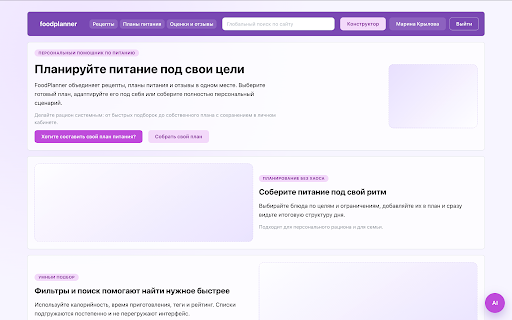
\includegraphics[width=0.95\textwidth]{image_7.png}
  }{
    \fbox{\parbox{0.9\textwidth}{\centering Место для изображения главной страницы\\
    Файл: \texttt{Report/images/image_7.png}}}
  }
  \caption{Главная страница приложения}
  \label{fig:image_7}
\end{figure}

Раздел рецептов реализует каталог с возможностью фильтрации по ключевым параметрам питания и кулинарного процесса. Пользователь может формировать релевантную выборку рецептов по тегам, калорийности, времени приготовления и другим критериям. Использование серверной фильтрации и постраничной загрузки поддерживает высокую отзывчивость интерфейса при росте объема данных.

Дополнительно реализована логика корректного отображения элементов пагинации: кнопка <<Показать еще>> отображается только при наличии данных для следующей подгрузки. Карточки рецептов содержат ключевые атрибуты для первичного выбора: название, краткое описание, теги, время приготовления и базовые показатели. Интерфейс раздела рецептов представлен на рисунке~\ref{fig:image_8}.

\begin{figure}[H]
  \centering
  \IfFileExists{images/image_8.png}{
    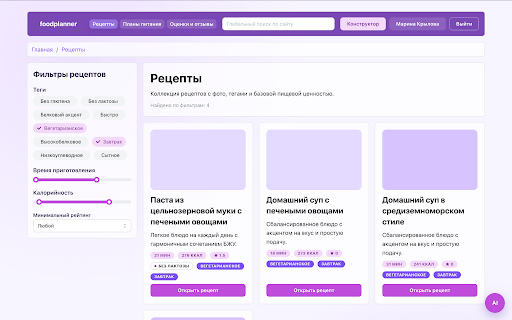
\includegraphics[width=0.95\textwidth]{image_8.png}
  }{
    \fbox{\parbox{0.9\textwidth}{\centering Место для изображения страницы рецептов\\
    Файл: \texttt{Report/images/image_8.png}}}
  }
  \caption{Страница рецептов}
  \label{fig:image_8}
\end{figure}

Детальная страница рецепта объединяет информационный и прикладной контуры. Информационный блок включает название, описание, пищевую ценность (калории, белки, жиры, углеводы), теги и пошаговую инструкцию. Прикладной блок реализует интерактивные действия: управление ингредиентами, формирование списка покупок, сохранение в профиль и экспорт.

Особое значение имеет блок ингредиентов с чекбоксами: пользователь отмечает наличие позиций, после чего система формирует список недостающих покупок. При повторном посещении страницы состояние чекбоксов восстанавливается, что поддерживает непрерывность пользовательского сценария. Детальная страница рецепта представлена на рисунке~\ref{fig:image_9}.

\begin{figure}[H]
  \centering
  \IfFileExists{images/image_9.png}{
    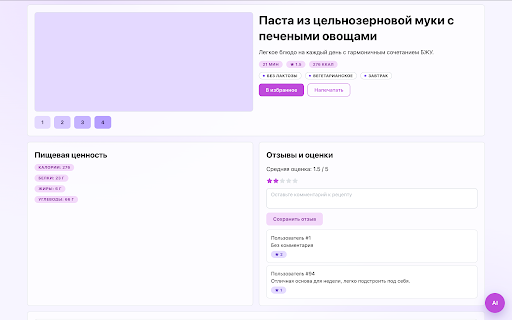
\includegraphics[width=0.95\textwidth]{image_9.png}
  }{
    \fbox{\parbox{0.9\textwidth}{\centering Место для изображения детальной страницы рецепта\\
    Файл: \texttt{Report/images/image_9.png}}}
  }
  \caption{Страница конкретного рецепта}
  \label{fig:image_9}
\end{figure}

Раздел планов питания является витриной готовых рационов и ориентирован на задачу быстрого выбора стратегии питания. Пользователь получает список планов с фильтрацией по типу, калорийности, рейтингу и дополнительным параметрам, включая персонализированные предпочтения. Серверная пагинация позволяет обрабатывать большие массивы данных без перегрузки интерфейса.

Карточка плана содержит ключевые характеристики для принятия решения: автор, тип плана, длительность, агрегированные показатели и оценка. Унификация карточек между разделами сокращает порог обучения и обеспечивает консистентный пользовательский опыт. Интерфейс страницы планов питания представлен на рисунке~\ref{fig:image_10}.

\begin{figure}[H]
  \centering
  \IfFileExists{images/image_10.png}{
    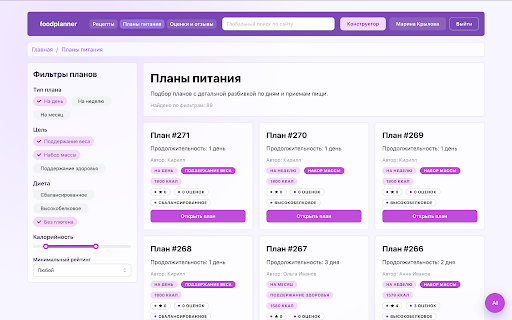
\includegraphics[width=0.95\textwidth]{image_10.png}
  }{
    \fbox{\parbox{0.9\textwidth}{\centering Место для изображения страницы планов питания\\
    Файл: \texttt{Report/images/image_10.png}}}
  }
  \caption{Страница планов питания}
  \label{fig:image_10}
\end{figure}

Детальная страница плана питания раскрывает структуру рациона по дням и приемам пищи (завтрак, обед, ужин, перекусы) с привязкой к рецептам и пищевым параметрам. Такой формат позволяет оценить рацион не только по агрегированным показателям, но и на уровне практического применения по каждому дню.

Интерфейс поддерживает раскрывающиеся секции и группировку данных, что упрощает навигацию внутри длинных планов и снижает визуальный шум. Как и на странице рецепта, доступны действия прикладного уровня: работа с ингредиентами, формирование списка покупок и сохранение результатов. Детальная страница плана питания представлена на рисунке~\ref{fig:image_11}.

\begin{figure}[H]
  \centering
  \IfFileExists{images/image_11.png}{
    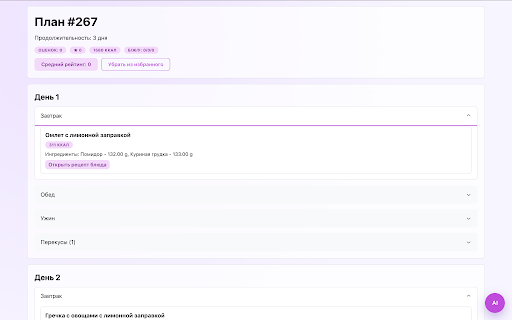
\includegraphics[width=0.95\textwidth]{image_11.png}
  }{
    \fbox{\parbox{0.9\textwidth}{\centering Место для изображения детальной страницы плана\\
    Файл: \texttt{Report/images/image_11.png}}}
  }
  \caption{Страница конкретного плана питания}
  \label{fig:image_11}
\end{figure}

Конструктор является центральным функциональным модулем приложения и предназначен для создания персонализированных планов питания. Интерфейс позволяет задавать параметры плана, выбирать рецепты из каталога и распределять их по календарной структуре. Реализована визуальная сегментация дней и поддержка вариативного количества перекусов.

Пользователь одновременно видит доступный контент и текущую структуру плана, что упрощает составление и корректировку рациона. По завершении формирования план отправляется на модерацию, после чего рабочая область конструктора подготавливается к следующему сценарию. Интерфейс конструктора представлен на рисунке~\ref{fig:image_12}.

\begin{figure}[H]
  \centering
  \IfFileExists{images/image_12.png}{
    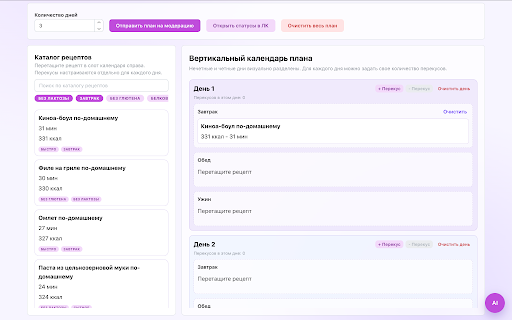
\includegraphics[width=0.95\textwidth]{image_12.png}
  }{
    \fbox{\parbox{0.9\textwidth}{\centering Место для изображения конструктора плана\\
    Файл: \texttt{Report/images/image_12.png}}}
  }
  \caption{Страница конструктора плана питания}
  \label{fig:image_12}
\end{figure}

Кабинет модератора реализован как специализированный интерфейс принятия решений. Для модератора скрыты нерелевантные персональные блоки, а в фокус вынесены заявки на проверку. Это снижает информационный шум и поддерживает операционный характер работы.

В блоке модерации рецептов отображаются карточки материалов в статусе проверки с ключевыми метаданными: тип сущности, автор, дата подачи и название. Каждая карточка предоставляет действия одобрения/отклонения и переход к детальному просмотру. Интерфейс кабинета модератора представлен на рисунке~\ref{fig:image_13}.

\begin{figure}[H]
  \centering
  \IfFileExists{images/image_13.png}{
    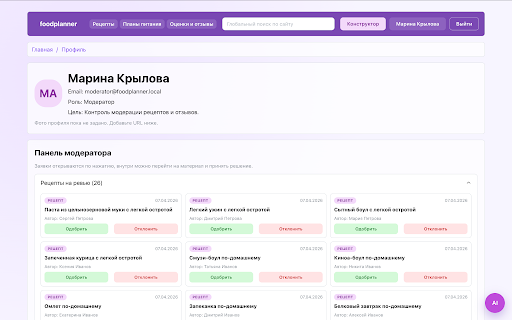
\includegraphics[width=0.95\textwidth]{image_13.png}
  }{
    \fbox{\parbox{0.9\textwidth}{\centering Место для изображения кабинета модератора\\
    Файл: \texttt{Report/images/image_13.png}}}
  }
  \caption{Личный кабинет модератора с модерацией}
  \label{fig:image_13}
\end{figure}

Личный кабинет пользователя предназначен для управления персональными данными и параметрами питания, влияющими на персонализацию контента. Пользователь может обновлять профиль, указывать цели, предпочтительную диету, особенности питания и любимые теги.

С точки зрения UX профиль построен как набор самостоятельных функциональных блоков: данные аккаунта, персональные предпочтения, избранное, собственные материалы, статусы модерации и связанные сущности (включая списки покупок). Поддержка пустых состояний и уведомлений о результате операций обеспечивает понятную обратную связь пользователю. Внешний вид личного кабинета пользователя представлен на рисунках~\ref{fig:image_14} и~\ref{fig:image_15}.

\begin{figure}[H]
  \centering
  \IfFileExists{images/image_14.png}{
    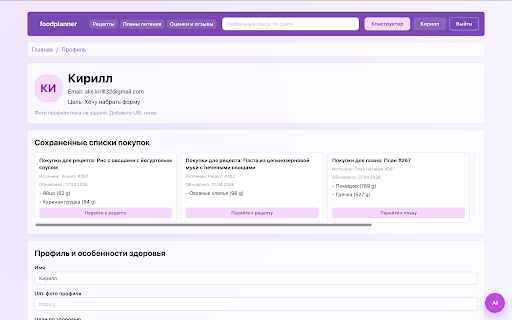
\includegraphics[width=0.95\textwidth]{image_14.png}
  }{
    \fbox{\parbox{0.9\textwidth}{\centering Место для изображения личного кабинета (вариант 1)\\
    Файл: \texttt{Report/images/image_14.png}}}
  }
  \caption{Личный кабинет пользователя}
  \label{fig:image_14}
\end{figure}

\begin{figure}[H]
  \centering
  \IfFileExists{images/image_15.png}{
    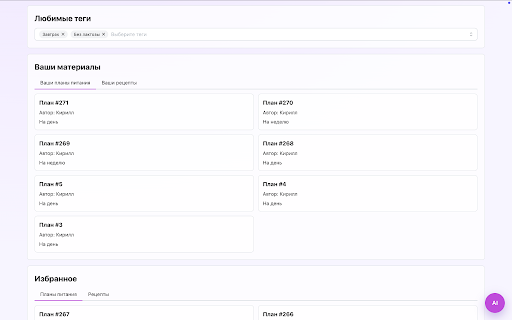
\includegraphics[width=0.95\textwidth]{image_15.png}
  }{
    \fbox{\parbox{0.9\textwidth}{\centering Место для изображения личного кабинета (вариант 2)\\
    Файл: \texttt{Report/images/image_15.png}}}
  }
  \caption{Личный кабинет пользователя}
  \label{fig:image_15}
\end{figure}

ИИ-ассистент интегрирован в приложение как доступный с любого экрана диалоговый интерфейс. Пользователь может открыть чат через плавающую кнопку и получить консультацию по рациону, подбору блюд и общим вопросам питания. Реализация в формате выдвижной панели обеспечивает быстрый доступ к функции без прерывания основного пользовательского сценария.

Интерфейс чата включает историю сообщений, поле ввода с повышенной читаемостью и явные состояния отправки/ожидания ответа. Дополнительно реализовано форматирование длинных ответов и обработка системных ошибок внешнего API через уведомления. Открытое диалоговое окно с ИИ-ассистентом представлено на рисунке~\ref{fig:image_16}.

\begin{figure}[H]
  \centering
  \IfFileExists{images/image_16.png}{
    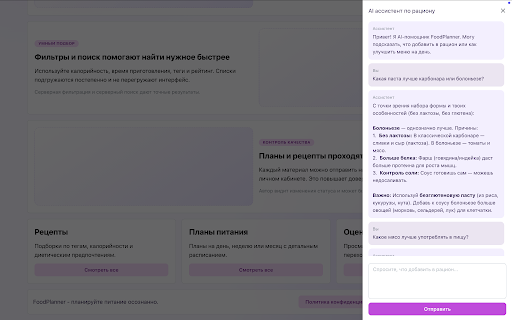
\includegraphics[width=0.95\textwidth]{image_16.png}
  }{
    \fbox{\parbox{0.9\textwidth}{\centering Место для изображения окна ИИ-ассистента\\
    Файл: \texttt{Report/images/image_16.png}}}
  }
  \caption{Открытое диалоговое окно с ИИ-ассистентом}
  \label{fig:image_16}
\end{figure}

Раздел оценок и отзывов обеспечивает прозрачный механизм социальной валидации контента. Пользователь может анализировать оценки и текстовые комментарии других участников платформы, что повышает доверие к опубликованным материалам и помогает принимать обоснованные решения при выборе рецептов и планов питания.

Функционально раздел агрегирует пользовательский опыт и одновременно является каналом обратной связи для авторов контента и модераторов. Интерфейс экрана реализован в формате карточек и списков с акцентом на читаемость комментариев, рейтинг и связь с объектом оценки. Страница оценок и отзывов представлена на рисунке~\ref{fig:image_17}.

\begin{figure}[H]
  \centering
  \IfFileExists{images/image_17.png}{
    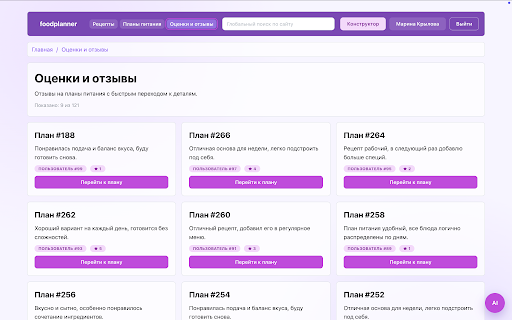
\includegraphics[width=0.95\textwidth]{image_17.png}
  }{
    \fbox{\parbox{0.9\textwidth}{\centering Место для изображения страницы оценок и отзывов\\
    Файл: \texttt{Report/images/image_17.png}}}
  }
  \caption{Страница оценок и отзывов}
  \label{fig:image_17}
\end{figure}

\section{Техническая реализация серверной части}

Информация о выборе архитектурного подхода и программных средств приведена в разделе~1.7. В данном разделе рассматриваются практические аспекты непосредственной серверной разработки: структура проекта, организация слоев ответственности, работа с базой данных, реализация API и поддержка ключевых бизнес-процессов.

Серверная часть FoodPlanner реализована на языке Python с использованием Django и Django REST Framework. Такой выбор позволил реализовать прикладную логику в сжатые сроки и при этом сохранить высокий уровень структурированности кода. В качестве основной СУБД используется PostgreSQL; для локальной отладки и быстрых проверок может использоваться SQLite.

Структура директории проекта серверной части. Серверный код размещен в директории \texttt{Backend} и организован по доменным приложениям. Каждое приложение изолирует отдельную часть предметной области и имеет собственные модели, сериализаторы, представления и маршруты. Ниже приведено назначение ключевых директорий:
\begin{compactlist}
  \item \texttt{/Backend} --- корневая директория серверной части, содержащая конфигурацию проекта, доменные модули, миграции и инфраструктурные файлы;
  \item \texttt{/Backend/config} --- модуль глобальной конфигурации: параметры Django, middleware, CORS/CSRF, подключение приложений, верхнеуровневые URL и служебные endpoint'ы;
  \item \texttt{/Backend/users} --- модуль пользователей и ролей: регистрация, вход/выход, профиль, ролевой доступ;
  \item \texttt{/Backend/recipes} --- модуль рецептов и справочников: категории, теги, ингредиенты, рецепты, фильтрация и модерационные действия;
  \item \texttt{/Backend/meal\_plans} --- модуль планов питания и shopping list: создание, редактирование, отправка на модерацию, детализация по дням и приемам пищи;
  \item \texttt{/Backend/interactions} --- модуль пользовательских взаимодействий: отзывы, оценки, жалобы, избранное;
  \item \texttt{/Backend/notifications} --- модуль уведомлений по событиям платформы;
  \item \texttt{/Backend/moderation} --- модуль журналирования модерационных действий;
  \item \texttt{/Backend/assistant} --- модуль ИИ-ассистента: серверный прокси-запрос к внешнему LLM-провайдеру с обработкой ошибок и контекста;
  \item \texttt{/Backend/*/migrations} --- миграции схемы БД для каждого доменного приложения;
  \item \texttt{/Backend/users/management/commands} --- management-команды (в том числе \texttt{seed\_demo\_data}) для ускорения тестирования сценариев.
\end{compactlist}

Организация серверной части по указанным модулям обеспечивает разделение ответственности, упрощает тестирование и снижает стоимость последующих изменений. Структура серверной части представлена на рисунке~\ref{fig:image_18}.

\begin{figure}[H]
  \centering
  \IfFileExists{images/image_18.png}{
    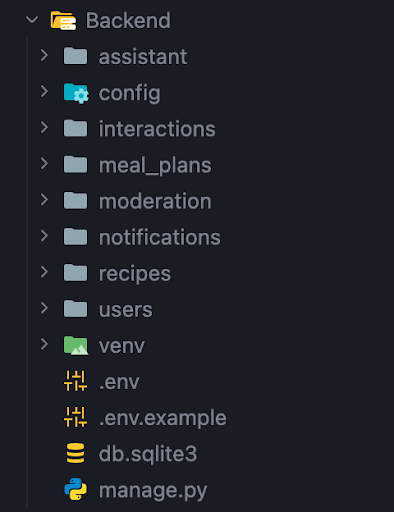
\includegraphics[width=0.95\textwidth]{image_18.png}
  }{
    \fbox{\parbox{0.9\textwidth}{\centering Место для изображения структуры серверной части\\
    Файл: \texttt{Report/images/image_18.png}}}
  }
  \caption{Структура серверной части проекта}
  \label{fig:image_18}
\end{figure}

Слойная организация серверной логики. Серверная часть построена по принципу разделения ответственности между тремя уровнями:
\begin{compactlist}
  \item уровень API (views/viewsets + serializers) --- прием входящих запросов, валидация формата данных, маршрутизация, формирование ответов;
  \item уровень бизнес-логики (доменные правила в приложениях, permissions, actions) --- реализация прикладных сценариев, проверка прав доступа, обработка статусов модерации и переходов жизненного цикла сущностей;
  \item уровень данных (models + ORM + migrations) --- описание структуры БД, связей, ограничений целостности, индексов и миграций.
\end{compactlist}

Такая модель не допускает концентрации всей логики в одном слое: API-уровень отвечает за протокол взаимодействия, доменный уровень --- за поведение системы, а модельный уровень --- за целостность хранения данных.

Реализация API и ключевые серверные сценарии. Сервер предоставляет REST API для всех основных ролей и пользовательских сценариев платформы. Ключевые контуры API включают:
\begin{compactlist}
  \item пользователей и профиль (регистрация, авторизация, выход, чтение и обновление профиля);
  \item рецепты (каталог, фильтрация, поиск, детальная карточка, модерация);
  \item планы питания (создание, редактирование, отправка на модерацию, решение модератора);
  \item отзывы и оценки (создание, изменение, модерация);
  \item жалобы и избранное (подача и обработка жалоб, пользовательские коллекции);
  \item списки покупок (формирование из рецепта/плана и сохранение в профиль);
  \item уведомления по событиям модерации и пользовательским действиям;
  \item ИИ-ассистент через безопасный backend-proxy endpoint.
\end{compactlist}

Работа с базой данных и моделью данных. В рассматриваемом проекте взаимодействие с БД реализовано преимущественно через Django ORM. В отличие от подхода с полностью ручным формированием SQL-запросов, ORM-подход был выбран осознанно и обусловлен следующими факторами:
\begin{compactlist}
  \item повышение скорости и надежности разработки за счет типовых операций чтения/записи без дублирования SQL-кода;
  \item единообразие и предсказуемость доступа к данным во всех доменных модулях проекта;
  \item снижение вероятности ошибок в CRUD-операциях и упрощение сопровождения при изменении схемы.
\end{compactlist}

Использование ORM в проекте не исключает контроля производительности. Для ресурсоемких сценариев применяются индексы, ограничения целостности, оптимизация выборок через механизмы ORM и явное проектирование связей между сущностями. Такая комбинация позволяет сохранить баланс между удобством разработки и эффективностью выполнения запросов.

Модель данных включает сущности пользователей, ролей, рецептов, ингредиентов, планов питания, элементов плана, отзывов, жалоб, избранного, уведомлений, списков покупок и журналов модерации. Между сущностями используются связи <<один-ко-многим>> и <<многие-ко-многим>>, что позволяет корректно покрывать прикладные сценарии.

Для критичных направлений (поиск, модерация, привязка shopping list к источнику, контроль уникальности взаимодействий) введены ограничения целостности и индексы. Миграции фиксируют эволюцию схемы БД и обеспечивают воспроизводимое развертывание на разных окружениях.

Хранение прикладных данных и медиа. Основные транзакционные данные (профили, рецепты, планы, отзывы, жалобы, уведомления) сохраняются в PostgreSQL. Файловые ресурсы в текущей версии могут размещаться в файловой системе сервера, что достаточно для учебного и пилотного контура эксплуатации. При переходе к промышленной эксплуатации архитектура допускает перенос медиа-ресурсов в объектное S3-совместимое хранилище без изменения прикладной бизнес-логики, за счет абстракции слоя хранения.

Пример получения пользователя при авторизации через сериализатор DRF приведен в листинге~\ref{listing:user-auth-lookup}. В отличие от ручного сравнения паролей в SQL-запросе, в проекте используется встроенный механизм \texttt{authenticate}, который учитывает хеширование паролей и backend-аутентификации Django.

\begin{listing}[H]
\caption{Проверка учетных данных пользователя при входе}
\label{listing:user-auth-lookup}
\begin{mdframed}
\begin{minted}[breaklines=true]{python}
class LoginSerializer(serializers.Serializer):
    email = serializers.EmailField()
    password = serializers.CharField(write_only=True)

    def validate(self, attrs):
        user = authenticate(
            request=self.context.get("request"),
            username=attrs["email"],
            password=attrs["password"],
        )
        if not user:
            raise serializers.ValidationError("Invalid credentials.")
        attrs["user"] = user
        return attrs
\end{minted}
\end{mdframed}
\end{listing}

Конфигурация подключения к базе данных определяется централизованно через настройки приложения и переменные окружения (листинг~\ref{listing:db-settings-singleton-analog}). Такой подход выполняет ту же функцию, что и ручная singleton-инициализация подключения в других стеках, но в терминах Django и его жизненного цикла.

\begin{listing}[H]
\caption{Конфигурация подключения к PostgreSQL в Django}
\label{listing:db-settings-singleton-analog}
\begin{mdframed}
\begin{minted}[breaklines=true]{python}
if env("POSTGRES_DB", default=""):
    DATABASES = {
        "default": {
            "ENGINE": "django.db.backends.postgresql",
            "NAME": env("POSTGRES_DB"),
            "USER": env("POSTGRES_USER", default="postgres"),
            "PASSWORD": env("POSTGRES_PASSWORD", default="postgres"),
            "HOST": env("POSTGRES_HOST", default="localhost"),
            "PORT": env("POSTGRES_PORT", default="5432"),
        }
    }
else:
    DATABASES = {
        "default": {
            "ENGINE": "django.db.backends.sqlite3",
            "NAME": BASE_DIR / "db.sqlite3",
        }
    }
\end{minted}
\end{mdframed}
\end{listing}

Использование переменных окружения является обязательной частью конфигурации backend. Переменные хранят параметры подключения, секретные ключи и настройки окружения без их жесткого встраивания в исходный код. Это повышает безопасность и позволяет использовать различные значения для разработки и production-среды (листинг~\ref{listing:env-loading}).

\begin{listing}[H]
\caption{Загрузка переменных окружения в настройках backend}
\label{listing:env-loading}
\begin{mdframed}
\begin{minted}[breaklines=true]{python}
import environ

BASE_DIR = Path(__file__).resolve().parent.parent
env = environ.Env(
    DEBUG=(bool, True),
    SECRET_KEY=(str, "django-insecure-change-me"),
)
environ.Env.read_env(BASE_DIR / ".env")

DEBUG = env("DEBUG")
SECRET_KEY = env("SECRET_KEY")
\end{minted}
\end{mdframed}
\end{listing}

Персонализация и серверная фильтрация. Одной из ключевых задач backend является выдача релевантных рецептов и планов питания с учетом параметров профиля (цели, теги, особенности питания). Фильтрация и пагинация реализованы на сервере, что обеспечивает:
\begin{compactlist}
  \item корректную обработку больших выборок;
  \item снижение нагрузки на клиент;
  \item единый источник правды по составу результатов;
  \item стабильное поведение интерфейса при комбинировании фильтров.
\end{compactlist}

Модерация как самостоятельный процесс. Модерационный контур реализован отдельно от пользовательского потока: пользователь создает контент и отправляет его на проверку, модератор или администратор принимает решение, после чего статус сущности обновляется и пользователю направляется уведомление. Такой подход обеспечивает управляемый жизненный цикл контента, аудит действий и масштабируемость процесса при росте нагрузки.

Используемые внешние библиотеки. Практическая реализация серверной части опирается на следующие группы библиотек:
\begin{compactlist}
  \item Django/DRF --- веб-фреймворк и REST-интерфейс;
  \item psycopg --- драйвер подключения к PostgreSQL;
  \item drf-spectacular --- генерация OpenAPI/Swagger-схемы;
  \item django-cors-headers --- управление CORS-политиками;
  \item django-environ --- загрузка конфигурации из переменных окружения;
  \item gunicorn --- production WSGI-сервер;
  \item стандартные модули Python для сетевого взаимодействия с внешним API ИИ-ассистента.
\end{compactlist}

Описание конечных точек API. Взаимодействие между клиентской и серверной частями реализовано в стиле REST с использованием протокола HTTP. Обмен данными строится на стандартных методах:
\begin{compactlist}
  \item \texttt{GET} --- получение ресурса или коллекции ресурсов;
  \item \texttt{POST} --- создание ресурса или запуск прикладного действия;
  \item \texttt{PUT/PATCH} --- полное или частичное обновление существующего ресурса;
  \item \texttt{DELETE} --- удаление ресурса (или логическое удаление в рамках бизнес-логики).
\end{compactlist}

Каждой группе ресурсов соответствует набор endpoint'ов, объединенных общим префиксом \texttt{/api}. Для отладки и тестирования API на этапе разработки использовались Swagger-интерфейс (\texttt{/api/docs/}) и ручная проверка запросов в Insomnia/Postman.

Список ключевых endpoint'ов серверной части:
\begin{compactlist}
  \item аутентификация и профиль пользователя:
  \texttt{POST /api/users/register/},
  \texttt{POST /api/users/login/},
  \texttt{POST /api/users/logout/},
  \texttt{GET/PATCH /api/users/me/};
  \item администрирование пользователей:
  \texttt{GET/POST /api/users/manage/},
  \texttt{GET/PATCH/DELETE /api/users/manage/\{id\}/};
  \item рецепты и справочники:
  \texttt{GET/POST /api/recipes/},
  \texttt{GET/PATCH/DELETE /api/recipes/\{id\}/},
  \texttt{POST /api/recipes/\{id\}/moderate/},
  \texttt{GET /api/recipes/categories/},
  \texttt{GET /api/recipes/ingredients/},
  \texttt{GET /api/recipes/tags/};
  \item планы питания и списки покупок:
  \texttt{GET/POST /api/meal-plans/},
  \texttt{GET/PATCH/DELETE /api/meal-plans/\{id\}/},
  \texttt{POST /api/meal-plans/\{id\}/submit\_for\_moderation/},
  \texttt{POST /api/meal-plans/\{id\}/moderate/},
  \texttt{GET/POST /api/meal-plans/shopping-lists/},
  \texttt{POST /api/meal-plans/shopping-lists/sync-target/};
  \item пользовательские взаимодействия:
  \texttt{GET/POST /api/interactions/reviews/},
  \texttt{POST /api/interactions/reviews/\{id\}/moderate/},
  \texttt{GET/POST /api/interactions/complaints/},
  \texttt{POST /api/interactions/complaints/\{id\}/resolve/},
  \texttt{GET/POST /api/interactions/favorites/};
  \item уведомления и ассистент:
  \texttt{GET /api/notifications/},
  \texttt{POST /api/notifications/\{id\}/mark\_read/},
  \texttt{POST /api/assistant/chat/};
  \item служебные endpoint'ы:
  \texttt{GET /api/health/},
  \texttt{GET /api/schema/},
  \texttt{GET /api/docs/}.
\end{compactlist}

\section{Техническая реализация клиентской части}

Клиентская часть FoodPlanner реализована как одностраничное веб-приложение (SPA) на React + TypeScript. Выбор данного подхода обусловлен необходимостью обеспечить быстрый отклик интерфейса, типобезопасность при работе с данными API и удобство развития проекта при добавлении новых пользовательских сценариев.

В качестве UI-библиотеки используется Mantine, которая предоставляет готовые адаптивные компоненты и упрощает поддержку единого визуального стиля. Для управления состоянием применен Effector, позволяющий явно описывать события, эффекты и зависимости между состояниями.

Структура проекта клиентской части. Код приложения организован по модульному принципу, где каждый каталог отвечает за ограниченную область ответственности:
\begin{compactlist}
  \item \texttt{/Frontend/src/pages} --- страницы верхнего уровня (маршруты пользовательского интерфейса);
  \item \texttt{/Frontend/src/components} --- переиспользуемые компоненты каркаса и представления;
  \item \texttt{/Frontend/src/features} --- feature-модули со сценарием и состоянием (например, аутентификация, профиль, конструктор плана);
  \item \texttt{/Frontend/src/shared/api} --- централизованный слой HTTP-взаимодействия с backend и обработка ошибок;
  \item \texttt{/Frontend/src/shared/ui} --- общие UI-блоки (уведомления, виджет ассистента, состояния загрузки/пустых данных);
  \item \texttt{/Frontend/src/shared/model} --- общие клиентские модели и события;
  \item \texttt{/Frontend/src/types} --- доменные типы и DTO-представления данных.
\end{compactlist}

Структура проекта клиентской части представлена на рисунке~\ref{fig:image_19}.

\begin{figure}[H]
  \centering
  \IfFileExists{images/image_19.png}{
    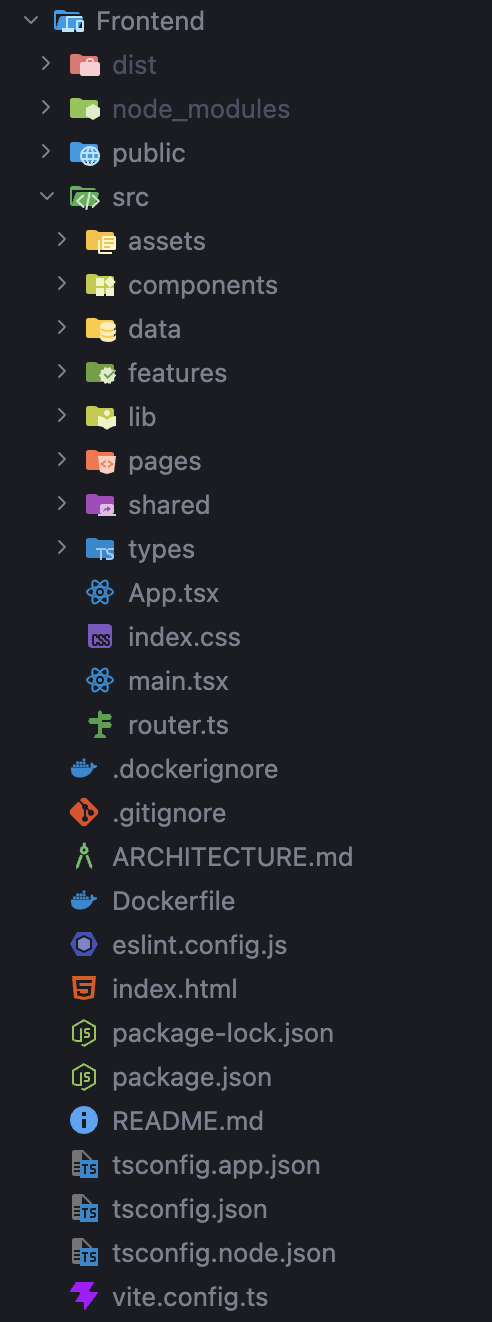
\includegraphics[width=0.95\textwidth]{image_19.png}
  }{
    \fbox{\parbox{0.9\textwidth}{\centering Место для изображения структуры клиентской части\\
    Файл: \texttt{Report/images/image_19.png}}}
  }
  \caption{Структура проекта клиентской части}
  \label{fig:image_19}
\end{figure}

Слойная архитектура клиентского приложения включает:
\begin{compactlist}
  \item presentation layer --- React-страницы и компоненты визуализации;
  \item state layer --- модели Effector и локальные состояния интерфейса;
  \item data access layer --- API-функции, инкапсулирующие HTTP-запросы, CSRF-защиту, преобразование DTO и обработку ошибок.
\end{compactlist}

Разработка экранов и навигации. Экранная структура клиентской части соответствует пользовательским сценариям, рассмотренным в разделе 2.1: каталог рецептов, карточка рецепта, планы питания, конструктор, отзывы, профиль и авторизация. Для маршрутизации используется \texttt{react-router-dom}; базовый набор маршрутов приложения приведен в листинге~\ref{listing:frontend-routing}.

\begin{listing}[H]
\caption{Маршрутизация экранов клиентской части}
\label{listing:frontend-routing}
\begin{mdframed}
\begin{minted}[breaklines=true]{tsx}
<Routes>
  <Route path="/" element={<AboutPage />} />
  <Route path="/auth" element={<AuthPage />} />
  <Route path="/recipes" element={<RecipesPage />} />
  <Route path="/recipes/:recipeId" element={<RecipeDetailPage />} />
  <Route path="/meal-plans" element={<MealPlansPage />} />
  <Route path="/meal-plans/:planId" element={<MealPlanDetailPage />} />
  <Route path="/reviews" element={<ReviewsPage />} />
  <Route path="/planner" element={<PlannerPage />} />
  <Route path="/profile" element={<ProfilePage />} />
  <Route path="*" element={<FallbackCard message="Страница не найдена." />} />
</Routes>
\end{minted}
\end{mdframed}
\end{listing}

Управление состоянием в клиентской части реализовано через Effector. Для аутентификации используются события пользовательских действий, асинхронные эффекты и производные состояния статуса сессии. Пример модели авторизации приведен в листинге~\ref{listing:frontend-auth-model}.

\begin{listing}[H]
\caption{Модель состояния аутентификации на Effector}
\label{listing:frontend-auth-model}
\begin{mdframed}
\begin{minted}[breaklines=true]{ts}
export const checkSessionRequested = createEvent()
export const loginSubmitted = createEvent<LoginPayload>()
export const logoutRequested = createEvent()

export const checkSessionFx = createEffect(async () => getMe())
export const loginFx = createEffect(async (payload: LoginPayload) => login(payload))
export const logoutFx = createEffect(async () => logout())

export const $authStatus = createStore<AuthStatus>('checking')
  .on(checkSessionFx.done, () => 'auth')
  .on(checkSessionFx.fail, () => 'guest')
  .on(loginFx.done, () => 'auth')
  .on(logoutFx.done, () => 'guest')

sample({ clock: checkSessionRequested, target: checkSessionFx })
sample({ clock: loginSubmitted, target: loginFx })
sample({ clock: logoutRequested, target: logoutFx })
\end{minted}
\end{mdframed}
\end{listing}

Интеграция с серверной частью построена через централизованный API-слой с единым форматом вызовов \texttt{GET/POST/PATCH/DELETE}. Для state-changing запросов используется CSRF-токен, а также включен режим \texttt{credentials: include} для корректной работы с сессионной аутентификацией. Фрагмент клиентского API-слоя приведен в листинге~\ref{listing:frontend-api-csrf}.

\begin{listing}[H]
\caption{Клиентский API-слой с CSRF-защитой}
\label{listing:frontend-api-csrf}
\begin{mdframed}
\begin{minted}[breaklines=true]{ts}
export async function ensureCsrfCookie() {
  if (getCookie('csrftoken')) return
  await fetch(`${API_BASE_URL}/health/`, { credentials: 'include' })
}

async function apiRequest<T>(path: string, method: 'GET' | 'POST' | 'PATCH', body?: unknown) {
  if (method !== 'GET') await ensureCsrfCookie()
  const csrfToken = getCookie('csrftoken')

  const response = await fetch(`${API_BASE_URL}${path}`, {
    method,
    credentials: 'include',
    headers: method === 'GET' ? undefined : {
      'Content-Type': 'application/json',
      'X-CSRFToken': csrfToken,
    },
    body: body ? JSON.stringify(body) : undefined,
  })

  if (!response.ok) throw await toApiError(response)
  return response.status === 204 ? (undefined as T) : ((await response.json()) as T)
}
\end{minted}
\end{mdframed}
\end{listing}

Дополнительным пользовательским сценарием является работа с ИИ-ассистентом: в интерфейсе реализован плавающий виджет с открытием боковой панели, сохранением истории диалога, отправкой сообщений через backend-proxy endpoint и обработкой ошибок с выводом уведомлений.

\section{Вывод}

Во второй главе рассмотрены практические аспекты технической реализации системы FoodPlanner. Описаны интерфейсные решения, серверная архитектура, организация клиентского и серверного кода, а также ключевые принципы интеграции между слоями приложения. Представленные решения обеспечивают функциональную полноту пользовательских сценариев и создают устойчивую основу для дальнейшего развития платформы.
\chapter{{\fontsize{14pt}{21pt}\selectfont\MakeUppercase{Тестирование, развертывание и внедрение системы}}}
\label{cha:testing}

\section{Тестирование системы}

Тестирование выполнено для подтверждения соответствия реализованного решения функциональным и нефункциональным требованиям, сформулированным в главе~1. Проверка включала серверную часть, клиентский интерфейс и интеграционные пользовательские сценарии.

Тестирование серверной части

Для backend-части (Django + DRF) использован модульный подход \cite{django_docs_2026,drf_docs_2026}:
\begin{compactlist}
  \item проверка корректности доменных моделей и ограничений целостности;
  \item проверка прав доступа по ролевой модели \texttt{user/moderator/admin};
  \item проверка сценариев модерации, обработки жалоб и уведомлений;
  \item проверка валидации входных данных и обработки ошибок API.
\end{compactlist}

Критериями приемки серверной части являются:
\begin{compactlist}
  \item успешное применение миграций и отсутствие конфликтов схемы БД;
  \item корректная работа основных API-методов (CRUD и служебные actions);
  \item отсутствие критических ошибок в системной проверке Django.
\end{compactlist}

Тестирование клиентской части

Для frontend-части (React + Effector) проведено функциональное тестирование ключевых пользовательских потоков \cite{react_docs_2026,effector_docs_2026}:
\begin{compactlist}
  \item авторизация и работа с профилем пользователя;
  \item просмотр и фильтрация каталогов рецептов и планов;
  \item формирование плана питания в конструкторе;
  \item работа с отзывами, избранным и списками покупок;
  \item обработка ошибок запросов и отображение уведомлений.
\end{compactlist}

Отдельно проверены граничные условия конструктора плана питания:
\begin{compactlist}
  \item длительность плана задается в диапазоне от 1 до 30 дней;
  \item шаг изменения длительности составляет 1 день;
  \item количество перекусов задается в диапазоне от 0 до 5 в сутки.
\end{compactlist}

Интеграционное тестирование

Интеграционная проверка выполнена на уровне бизнес-сценариев:
\begin{compactlist}
  \item регистрация пользователя и заполнение профиля;
  \item создание рецепта, отправка на модерацию, изменение статуса;
  \item формирование плана питания и генерация списка покупок;
  \item публикация отзыва, создание жалобы, получение уведомления;
  \item обращение к ИИ-ассистенту через серверный прокси.
\end{compactlist}

Результаты тестирования подтвердили работоспособность основных сценариев использования системы и согласованность работы клиентской и серверной частей.

\section{Развертывание на сервере}

Сборка и контейнеризация серверной части

Для унификации окружения и воспроизводимости развертывания приложение упаковано в Docker-контейнеры \cite{docker_docs_2026}. Проект включает:
\begin{compactlist}
  \item контейнер базы данных PostgreSQL;
  \item контейнер backend-сервиса (Django + Gunicorn);
  \item контейнер frontend-сервиса (Vite + React).
\end{compactlist}

Конфигурация backend-контейнера приведена в листинге~\ref{listing:backend-dockerfile}.

\begin{listing}[H]
\caption{Dockerfile серверной части}
\label{listing:backend-dockerfile}
\begin{mdframed}
\begin{minted}[breaklines=true]{bash}
FROM python:3.13-slim
ENV PYTHONDONTWRITEBYTECODE=1 PYTHONUNBUFFERED=1
WORKDIR /app
COPY requirements.txt /app/requirements.txt
RUN pip install --no-cache-dir -r /app/requirements.txt
COPY . /app
EXPOSE 8000
CMD ["gunicorn", "config.wsgi:application", "--bind", "0.0.0.0:8000"]
\end{minted}
\end{mdframed}
\end{listing}

Конфигурация frontend-контейнера приведена в листинге~\ref{listing:frontend-dockerfile}. Сборка выполняется через \texttt{npm ci}, а запуск dev-сервера --- через Vite \cite{npm_docs_2026,vite_docs_2026,vite_deploy_docs_2026}.

\begin{listing}[H]
\caption{Dockerfile клиентской части}
\label{listing:frontend-dockerfile}
\begin{mdframed}
\begin{minted}[breaklines=true]{bash}
FROM node:22-alpine
WORKDIR /app
COPY package.json package-lock.json /app/
RUN npm ci
COPY . /app
EXPOSE 5173
CMD ["npm", "run", "dev", "--", "--host", "0.0.0.0", "--port", "5173"]
\end{minted}
\end{mdframed}
\end{listing}

Оркестрация сервисов

Для запуска полного стенда используется \texttt{docker-compose.yml}, включающий базы данных, backend и frontend (листинг~\ref{listing:compose-file}) \cite{docker_compose_docs_2026}.

\begin{listing}[H]
\caption{Фрагмент docker-compose.yml}
\label{listing:compose-file}
\begin{mdframed}
\begin{minted}[breaklines=true]{yaml}
services:
  db:
    image: postgres:16-alpine
  backend:
    build: ./Backend
    ports: ["8000:8000"]
    command: >
      sh -c "python manage.py migrate &&
             gunicorn config.wsgi:application --bind 0.0.0.0:8000"
  frontend:
    build: ./Frontend
    ports: ["5173:5173"]
\end{minted}
\end{mdframed}
\end{listing}

Порядок запуска

Последовательность развертывания:
\begin{compactlist}
  \item перейти в корневую директорию проекта;
  \item скачать (при необходимости обновить) образы командой \texttt{docker compose pull};
  \item выполнить сборку контейнеров командой \texttt{docker compose build};
  \item запустить окружение командой \texttt{docker compose up -d};
  \item проверить доступность сервисов: frontend (\texttt{http://localhost:5173}), backend API (\texttt{http://localhost:8000/api/health/}).
\end{compactlist}

Такой подход сокращает время подготовки среды и обеспечивает идентичное поведение приложения на разных хостах.

\section{Перспективы развития системы}

Дальнейшее развитие FoodPlanner целесообразно выполнять по следующим направлениям:
\begin{compactlist}
  \item расширение доменной персонализации (сезонность, бюджет, расширенные медицинские ограничения);
  \item развитие рекомендательных алгоритмов и повышение качества ИИ-консультаций;
  \item интеграция с внешними сервисами (трекеры активности, носимые устройства, продуктовые каталоги);
  \item расширение аналитики пользовательского прогресса и поведенческих метрик;
  \item усиление контуров качества: автоматизированные e2e-тесты, CI/CD и централизованная телеметрия.
\end{compactlist}

\section{Выводы по главе}

В третьей главе представлены результаты тестирования, подтверждающие работоспособность ключевых пользовательских и служебных сценариев системы. Показано развертывание приложения в контейнерной среде Docker с использованием единого файла оркестрации сервисов. Также определены приоритетные направления дальнейшего развития, направленные на повышение качества персонализации, масштабируемости и эксплуатационной зрелости платформы.

\backmatter % Здесь заканчивается нумерованная часть документа и начинаются ссылки и заключение

\Conclusion % заключение к отчёту

Выполнение выпускной квалификационной работы базировалось на анализе предметной области, сравнительном исследовании существующих решений, проектировании архитектуры системы и практической реализации программного продукта.

В ходе выполнения работы были решены следующие задачи:
\begin{compactlist}
  \item выполнен анализ предметной области планирования питания и выявлены ключевые проблемы целевой аудитории;
  \item проведен анализ аналогов и конкурентов, определены ограничения существующих подходов;
  \item спроектированы бизнес-процессы и формализованы сценарии взаимодействия пользователей с системой;
  \item сформированы бизнес-, функциональные и нефункциональные требования к разрабатываемой системе;
  \item спроектирована архитектура веб-приложения и определена ролевая модель доступа;
  \item разработана структура базы данных и описаны связи доменных сущностей;
  \item разработаны макеты и реализован пользовательский интерфейс клиентской части;
  \item реализованы серверная и клиентская части приложения, включая контуры персонализации, модерации, отзывов, уведомлений и ИИ-ассистента;
  \item выполнено тестирование ключевых пользовательских и административных сценариев;
  \item описаны и реализованы подходы к контейнеризации и развертыванию системы.
\end{compactlist}

По результатам выполненной работы разработанное веб-приложение FoodPlanner демонстрирует работоспособность заявленных сценариев и может использоваться в качестве основы для дальнейшего внедрения и развития.

В качестве перспектив развития рассматриваются расширение аналитического контура, развитие инструментов модерации и администрирования, а также усиление персонализации рекомендаций на основе пользовательского поведения.

Таким образом, поставленные задачи решены, а цель выпускной квалификационной работы --- разработка веб-приложения для планирования питания с учетом предпочтений пользователей --- достигнута.



% % Список литературы при помощи BibTeX
% Юзать так:
%
% pdflatex rpz
% bibtex rpz
% pdflatex rpz


\nocite{
who2025stats,
povarenok2026,
eda2026,
myfitnesspal2026,
supercook2026,
ovkuse2026,
react_docs_2026,
typescript_docs_2026,
effector_docs_2026,
mantine_docs_2026,
python_docs_2026,
django_docs_2026,
drf_docs_2026,
postgresql_docs_2026,
docker_docs_2026,
docker_compose_docs_2026,
owasp_top10_2021,
owasp_csrf_cheatsheet,
owasp_xss_cheatsheet
}

\bibliographystyle{gost780u}
\bibliography{rpz}


%%% Local Variables:
%%% mode: latex
%%% TeX-master: "rpz"
%%% End:


% Тут идут приложения

\end{document}